% interactnlmsample.tex
% v1.05 - August 2017

\documentclass[]{interact}

\usepackage{epstopdf}% To incorporate .eps illustrations using PDFLaTeX, etc.


%\usepackage[caption=true]{subfig}% Support for small, `sub' figures and tables
%\usepackage[nolists,tablesfirst]{endfloat}% To `separate' figures and tables from text if required
%\usepackage[doublespacing]{setspace}% To produce a `double spaced' document if required
%\setlength\parindent{24pt}% To increase paragraph indentation when line spacing is doubled

\usepackage[noadjust]{cite}
\usepackage{graphicx}                
\usepackage{array,graphicx,float,caption}
\usepackage{subcaption}
\captionsetup{compatibility=false}
\usepackage{overpic}

\usepackage{booktabs}
\usepackage[normalem]{ulem}
% packages needed for Perla's commands
\usepackage{color}
\usepackage{soul}
\usepackage{array, amsmath}

\usepackage[numbers,sort&compress]{natbib}% Citation support using natbib.sty
\bibpunct[, ]{[}{]}{,}{n}{,}{,}% Citation support using natbib.sty
\renewcommand\bibfont{\fontsize{10}{12}\selectfont}% Bibliography support using natbib.sty
\makeatletter% @ becomes a letter
\def\NAT@def@citea{\def\@citea{\NAT@separator}}% Suppress spaces between citations using natbib.sty
\makeatother% @ becomes a symbol again

\theoremstyle{plain}% Theorem-like structures provided by amsthm.sty
\newtheorem{theorem}{Theorem}[section]
\newtheorem{lemma}[theorem]{Lemma}
\newtheorem{corollary}[theorem]{Corollary}
\newtheorem{proposition}[theorem]{Proposition}

\theoremstyle{definition}
\newtheorem{definition}[theorem]{Definition}
\newtheorem{example}[theorem]{Example}

\theoremstyle{remark}
\newtheorem{remark}{Remark}
\newtheorem{notation}{Notation}


\newcommand{\degree}{$^{\circ}$ }

\begin{document}

%Commands defined by Perla
\newcommand{\DelP}[1]{\textcolor{red}{\st{#1}}}
\newcommand{\AddP}[1]{\textcolor{blue}{#1}}
\newcommand{\NoteP}[1]{\textcolor{green}{#1}}
\newcommand{\ULsubfloat}[2][\empty]% #1 = caption (optional), #2 = image
%\articletype{ARTICLE TEMPLATE}% Specify the article type or omit as appropriate

\title{Effective Haptic Interactions for Information Self-Structuring}

%Motion Strategies For Autonomous Categorization of Hard Inclusions in Soft Body

\author{
\name{Luca Scimeca\thanks{CONTACT Luca Scimeca Author. Email: ls769@cam.ac.uk}, Perla Maiolino, Ed Bray and Fumiya Iida }
\affil{Bioinspired Robotic Lab, Engineering Department, University of Cambridge, Cambridge UK}
}

\maketitle

\begin{abstract}
This paper presents ....
We explore different robotic palpation strategies and we evaluate their capabilities to find invariant features (depth, size) of hard inclusions in a soft phantom.
We used PCA and KNN for clustering the data ...
The results show that ...
\end{abstract}

\begin{keywords}
Robotic palpation; Tactile sensor; hard nodule detection; 
\end{keywords}

\section{Introduction}

%Tactile sensor modalities play a fundamental role in biological systems.
In the last decades, substantial efforts have been made in enhancing the sensing capabilities of robots by providing them with a sense of touch \cite{dahiya_tactile_2010}. Haptic perception differs from other mechanisms in virtue of its tight coupling with, and need of, physical interactions. 

The coupling of motion and tactile sensing plays a crucial role in determining which tasks are more suited to the haptic framework, and directly influence the interaction strategy needed with the environment. In medical palpation diagnosis, for example, given the nature of the soft tissues in the body and the scarcity of helpful stimuli other than touch, haptic perception plays a fundamental role. Here, practitioners necessitate the use of different motion palpation strategies according to the palpation task, whether this is an organ to examine, finding hard (cancerous) inclusions or investigating their characteristics (cite paper). In the latter case, for instance, the richness of the stimuli when probing the soft body, and the complexity of the underlying principles that generated them, requires a mechanism both capable of categorizing such stimuli and coping with high dimensional information.

The need to categorize arises continuously throughout the life of many biological systems, where discriminating between different stimuli requires advanced sensory-motor coordination capabilities. In biological systems, categorization is the result of a dynamical interaction between the nervous system, the body and the environment \cite{Pfeifer1088}, where motor actions have an active role in determining the sensory pattern that is received. Understanding similarities or differences between stimuli from the world has instead been a challenge for machines since the dawn of robotics.  

The consequences of motion to the perceived stimuli have been the focus of much work in the past years, mainly showing how through the coordination of motor actions, it is possible to select or influence the perceived sensory patterns, actively improving the ability to retrieve information from the world and arguing in favor of the benefits of such ability to, for instance, appropriately categorize perceptual stimuli \AddP{cite Nolfi paper?}\cite{lungarella2005methods, sporns2006evolving, pfeifer2007information}. The change in information structure due to said interaction sets the context for what is known as information self-structuring \cite{pfeifer2007information}. 

As we will show, the influence of motion to the structuring of the information, however, can not be analyzed singularly, as its effect primarily depend on the environment, and consequently on the nature of the information itself and the quality and quantity of the data at hand. We refer to a cognitive map, as the representation of the categorical space, dividing the stimuli into their respective categories. 
%soft tissue non-linearities and complex interaction forces that can be produced during the exploratory motion, an additional layer of complexity to the discrimination task. 

%
%Categorization and recognition are fundamental cognitive activities in many biological systems, performed throughout their lifetime and requiring advanced sensory-motor coordination capabilities. Understanding similarities or differences between stimuli from the world has instead been a challenge for machines since the dawn of robotics.

%In its simplest form, recognition happens when a previously encountered stimulus is recognized as such, and discriminated between other, dissimilar, stimuli. The minimum requirement for recognition is thus a form of understanding of the stimulus, whose properties can be explicitly extracted and modeled or implicitly stored for comparison.  \AddP{paragraph on doing it with explicit modeling?}


This paper proposes an approach to obtain cognitive maps for the categorization of tactile stimuli. 
We explore the way motor induced physical interaction with a soft body affects the structure of haptic, spatiotemporal, information. 

%In the context of sensory-motor coordination, in fact, an additional layer of complexity is induced when interacting with a deformable (soft) body, whose dynamic properties are hard to model and its reactions to predict.
%The material non-linearities and complex interaction forces that can be produced during the exploratory motion, make the problem highly non-trivial. 

\begin{figure}[]
	\centering
	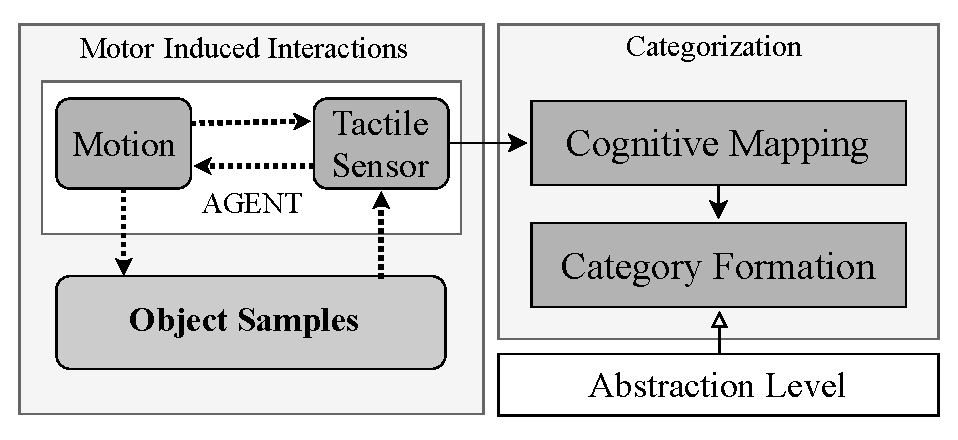
\includegraphics[width=0.64\textwidth]{./figs/conceptual_framework}
	\caption{Conceptual map for the Motion Primitive Pre-processing of Sensory Receptors.}
	\label{conceptual_map}
\end{figure}

In the context of sensory-motor coordination, the environment is here represented by a soft, elastic, phantom organ, containing various hard inclusions. The robot interacts with the organ by probing it at various locations (samples), thus influencing the sensor response and in turn the perceived tactile stimuli. From the stimuli, categories are formed and a cognitive map is retrieved (see Fig. \ref{conceptual_map}).

We use an unsupervised clustering method to enable an agent to automatically find structure in unstructured data. When interacting with a soft body through a sensorised probe, then, the motion strategy of the agent during interaction changes the sensory response of the interacting sensorised probe, modifying the retrieved data and consequently the discretization of the stimuli into clusters. The choice of the number of clusters to divide the space into is also an important influencing factor on the resulting categorization. By analyzing which motion influences the sensor response coherently with the finding of meaningful clusters for the task at hand, we can assess the relationship between motion and the underlying change in the agent's cluster perception. The use of an unsupervised learning technique is here fundamental, as it allows the agent to base the inference solely on the information pre-structured by the motion strategy, without influencing it in any active way.


As for the implication of the body, we have previously proposed a conceptual framework, based on unsupervised learning, to explore how sensor morphology can drive the robot's internal representation of the world. In particular we showed that change in sensor morphology processes the sensory response before a central processing system can make inference, and that the processing can actively be taken advantage of with respect to a task.

%Indeed supervised learning neural network, commonly used to associate the stimulus with the appropriate response, can face the problems of \textit{perceptual aliasing} (i.e., objects that require different reactions provide equivalent input to the system), and the inability to learn certain categories. 
%The problem can be significantly simplified if it is viewed as sensory-motor coordination


%Medical palpation is an essential clinical skill and a complex mechanical process that constitutes a part of a complete physical examinations which allows clinicians to perform accurate diagnosis. Palpation is usually used in breast and prostate examination in order to determine the presence of a hard nodule and, along with that, other characteristics such that location, dimension and mechanical properties. 


%This paper thus proposes a learning mechanism of robot motion to induce sensor stimuli to discriminate between inclusions in soft structures.

%The main contribution of this paper is to propose the same conceptual framework to examine whether any processing or $meaningful$ $transformations$ occur in robotic tactile sensing due to the performed probing motion, with the objective to detect hard inclusions in soft phantom. 
%Furthermore, we explore the usefulness of unsupervised learning to learn which is the best motion strategy for improving the detection accuracy of specific configuration of size and embedding depth of the hard inclusion. 


%In this respect, we consider a learning problem of tactile discrimination tasks, in which a robotic palpation system should acquire categories of tactile sensing information induced by different types of objects physically in contact. We consider these categories to be autonomously generated through unsupervised clustering of sensory information. The way in which the robot clusters the objects is related to how the objects' geometrical characteristics are perceived during the interactions.

For the experiments, we develop a sensorised probe provided with a new capacitive tactile sensor array with high spatial resolution \cite{schmitz_methods_2011}, we design a soft, elastic, phantom organ and set two different probing motions. 
During interaction with the soft phantom organ, the different type of motion utilized changes the sensor response. The altered sensory input directly influences the way in which the probed locations in the phantom are perceived and in turn their clustering. We simplify the scenario by choosing hard nodules of two different sizes and embed them in the phantom organs at two depths. Furthermore, we develop an unsupervised method to automatically interpret relations amongst the different probed locations, and observe how, when fixing the robot's inference strategy, we can affect its internal representations simply by changing the probing motion.


The paper is organized as follows: In Section \ref{sec_unsup_clustering} we describe the proposed unsupervised method for clustering using the soft filters, in Section \ref{sec_setup} we describe in detail the tactile sensor technology as well as the experimental set-up used for performing the experiments. In section \ref{sec_results} the experimental results are presented. Finally, section \ref{sec_discussion} gives a discussion of the results followed by a conclusion in Section \ref{sec_conclusion}.

% \section{Related Works}
% The majority of the previous research have been devoted to the development of probing systems based on various design and transduction principle (ref to Liza review paper). Only few works have been devoted to the exploration of different motions strategies to improve the efficiency of probing devices during artificial palpation (cite Liza works). In particular manual palpation techniques were studied in order to understand optimal control strategies for artificial palpation probe to detect hard nodules in soft tissues.

% \subsection{sensorised probe design}
% A review about the latest advancements and challenges in the development of tactile sensing palpation and probing devices can be found in. 
% Despite several devices have been developed tactile sensation is not yet broadly implemented for real surgical applications, as described in [4].
% One of the main reasons for that may be the strict certification requirements specified for medical devices.
% Requirements:
% \begin{itemize}
% \item the surgeon does not have the possibility to perform multiple tactile scans of an organ to confirm the presence or location of a tumor inside an organ. A
% probe for tactile data detection should ensure the possibility to measure soft tissue properties within a short period of time,
% \item accuracy and stability of the devices and their measurements
% \item robust to variability factors (breath, liquids)
% \item miniaturized, disposable, sterile
% \end{itemize}


% \subsection{localization}\label{localization}

% \subsection{Type of motion} \label{motion}
% There are several palpation techniques in use, depending on the organ examined and the shape and depth of the abnormality [41], [42]. Palpation methods can be subdivided into three main techniques, such as
% global movement, local movement and palpation pressure,
% though they are usually combined in order to achieve the best result [43]. 

% -global movement: Clinical breast examinations are usually performed with the following three patterns: concentric circles, radial spokes, and vertical stripes [45]. The pattern choice mainly depends on the preference and training of the examiner.
% -the local finger movement (LFM) method is applied, and performed only within a selected section. This type of palpation helps physicians to understand the shape and depth of an abnormality.  In particular, three methods of LFM can be
% outlined for palpation examinations performed with one finger
% [45]. The first method is tapping - a fast striking discontinuous touching of the tissue. The second technique is vibration, where the finger is kept at constant contact with the tissue and the force direction of the finger is varied during examination.
% Finally, there is the sliding pattern - a smooth movement over a defined area with relatively constant pressure. 
% -finger movement pressure (FMP), which corresponds to the average intentional finger pressure applied during the palpation procedure, such as light and deep palpation [46].
% Light pressure is mainly used with GFM to access the general mechanical properties and temperature of the organs.
% Indentation of this type of palpation does not exceed 2 cm and
% pressure is as light as possible. Deep palpation is performed
% with heavier pressure, mainly used for LFM, with an
% indentation of about 4 cm, and is used to evaluate the stiffness,
% size, contours and shape of the formation or of the organ. 

\section{Methods}

In this section we list the proposed framework, the reference tactile sensor technology, the selected motions strategies and the robot setup used for performing the experiments.

%We investigate the influence of different palpation motions have on tactile information encoding and so in detection on hard nodules.
\subsection{Reference Tactile Sensor Technology and Data Acquisition} \label{sec_setup}


The reference tactile sensor technology has been described in \cite{schmitz_methods_2011}. The adopted sensing mode is based on the capacitive transduction principle. A capacitive transducer (i.e., a tactile element, or $taxel$) is organized in a layered structure: the lower layer consists of the positive electrode, which is mounted on a Flexible Printed Circuit Board (FPCB); a small air chamber act as dielectric and the upper layer is a ground plane made with conductive lycra. The tactile sensor is made up of a number of taxels geometrically organized in triangular modules (Fig. \ref{CySkin:skin}). 

In the current prototype, each module hosts $7$ taxels, as well as the Capacitance to Digital Converter (CDC) chip (namely, the AD7147 from Analog Devices) for converting capacitance values to digital. The CDC chip can measure variations in capacitance values with 16 bits of resolution. All the modules are interconnected and communicate through an SPI bus to a read-out board which perform a preliminary processing of the tactile sensor data and send them to the PC through CAN bus (Fig. \ref{CySkin:schema}). %within the $4 \div 30pF$ range with a sensitivity of $0.32fF$. 
In this context, the normal forces exerted on the sensor produce variations in capacitance values reflecting the varied pressure over the taxel positions. A sensor reading, or tactile image, from the tactile sensor described is produced at $20Hz$, and corresponds to a 7-dimensional array, where each element contains the capacitance variation value of the corresponding taxel (Fig. \ref{CySkin:skin}).
%is $\Delta C_i$, and $i$ is its corresponding taxel in the sensor.
When performing the experiments, the  tactile images are seldom used singularly. For every motion strategy designed, we take sensor readings in sequence over equally spaced intervals, varying with the motion strategy, and concatenate them sequentially into a single array (time series).
In this paper we refer to a tactile image sequence as the concatenated sensor readings after applying a specific motion strategy.
To carry out the experiments we design and 3d-print a set of hard inclusions to embed in the soft phantom.
\begin{figure}[]
	\centering
	\begin{subfigure}[b]{.65\textwidth}
		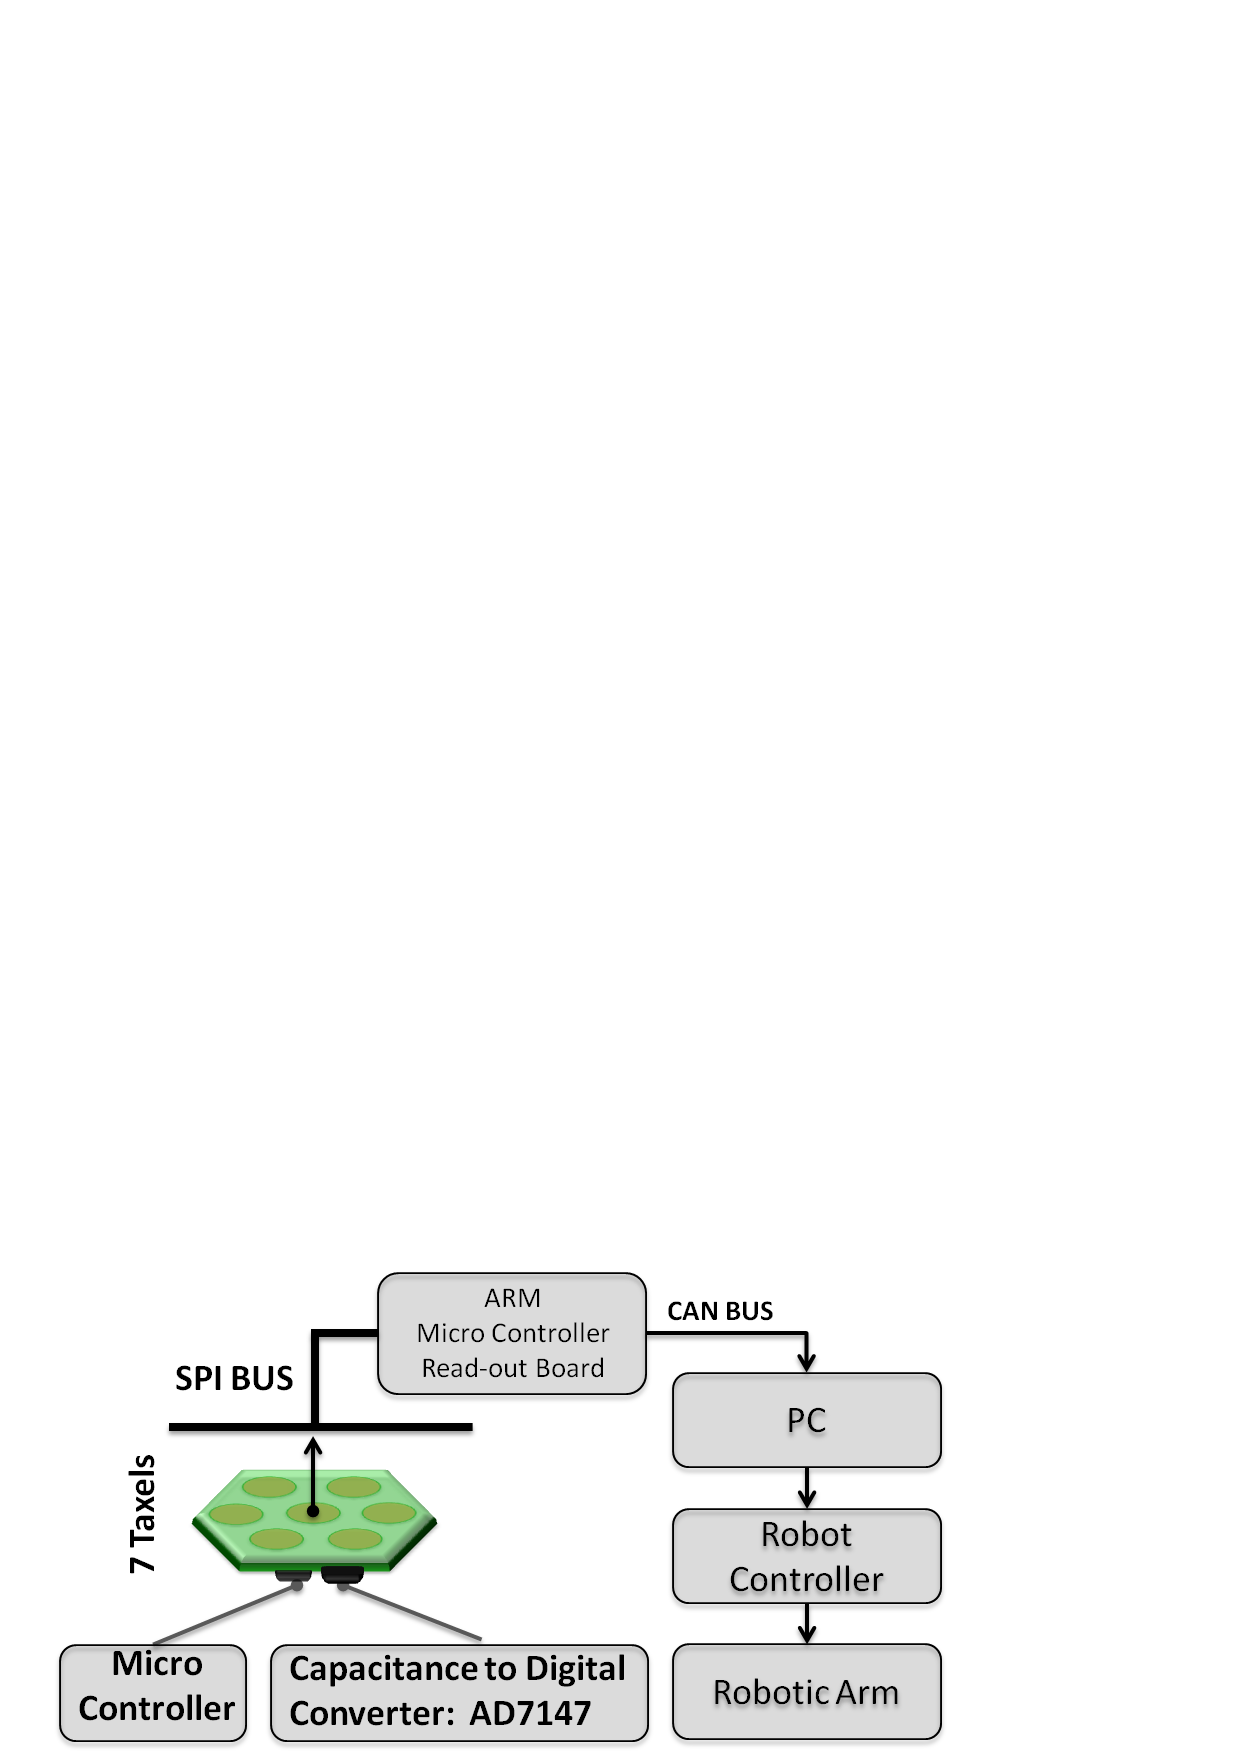
\includegraphics[width=\textwidth]{./figs/Presentationarchitecture.pdf}
		\caption{}
		\label{CySkin:schema}
	\end{subfigure} 
	\hspace{0.01\textwidth}
	\begin{subfigure}[b]{.51\textwidth}
		\includegraphics[width=\textwidth]{./figs/expsetupnew.jpg}
		\caption{}
		\label{exp:robot}
	\end{subfigure} 
	\hspace{0.01\textwidth}
	\begin{subfigure}[b]{0.32\textwidth}
		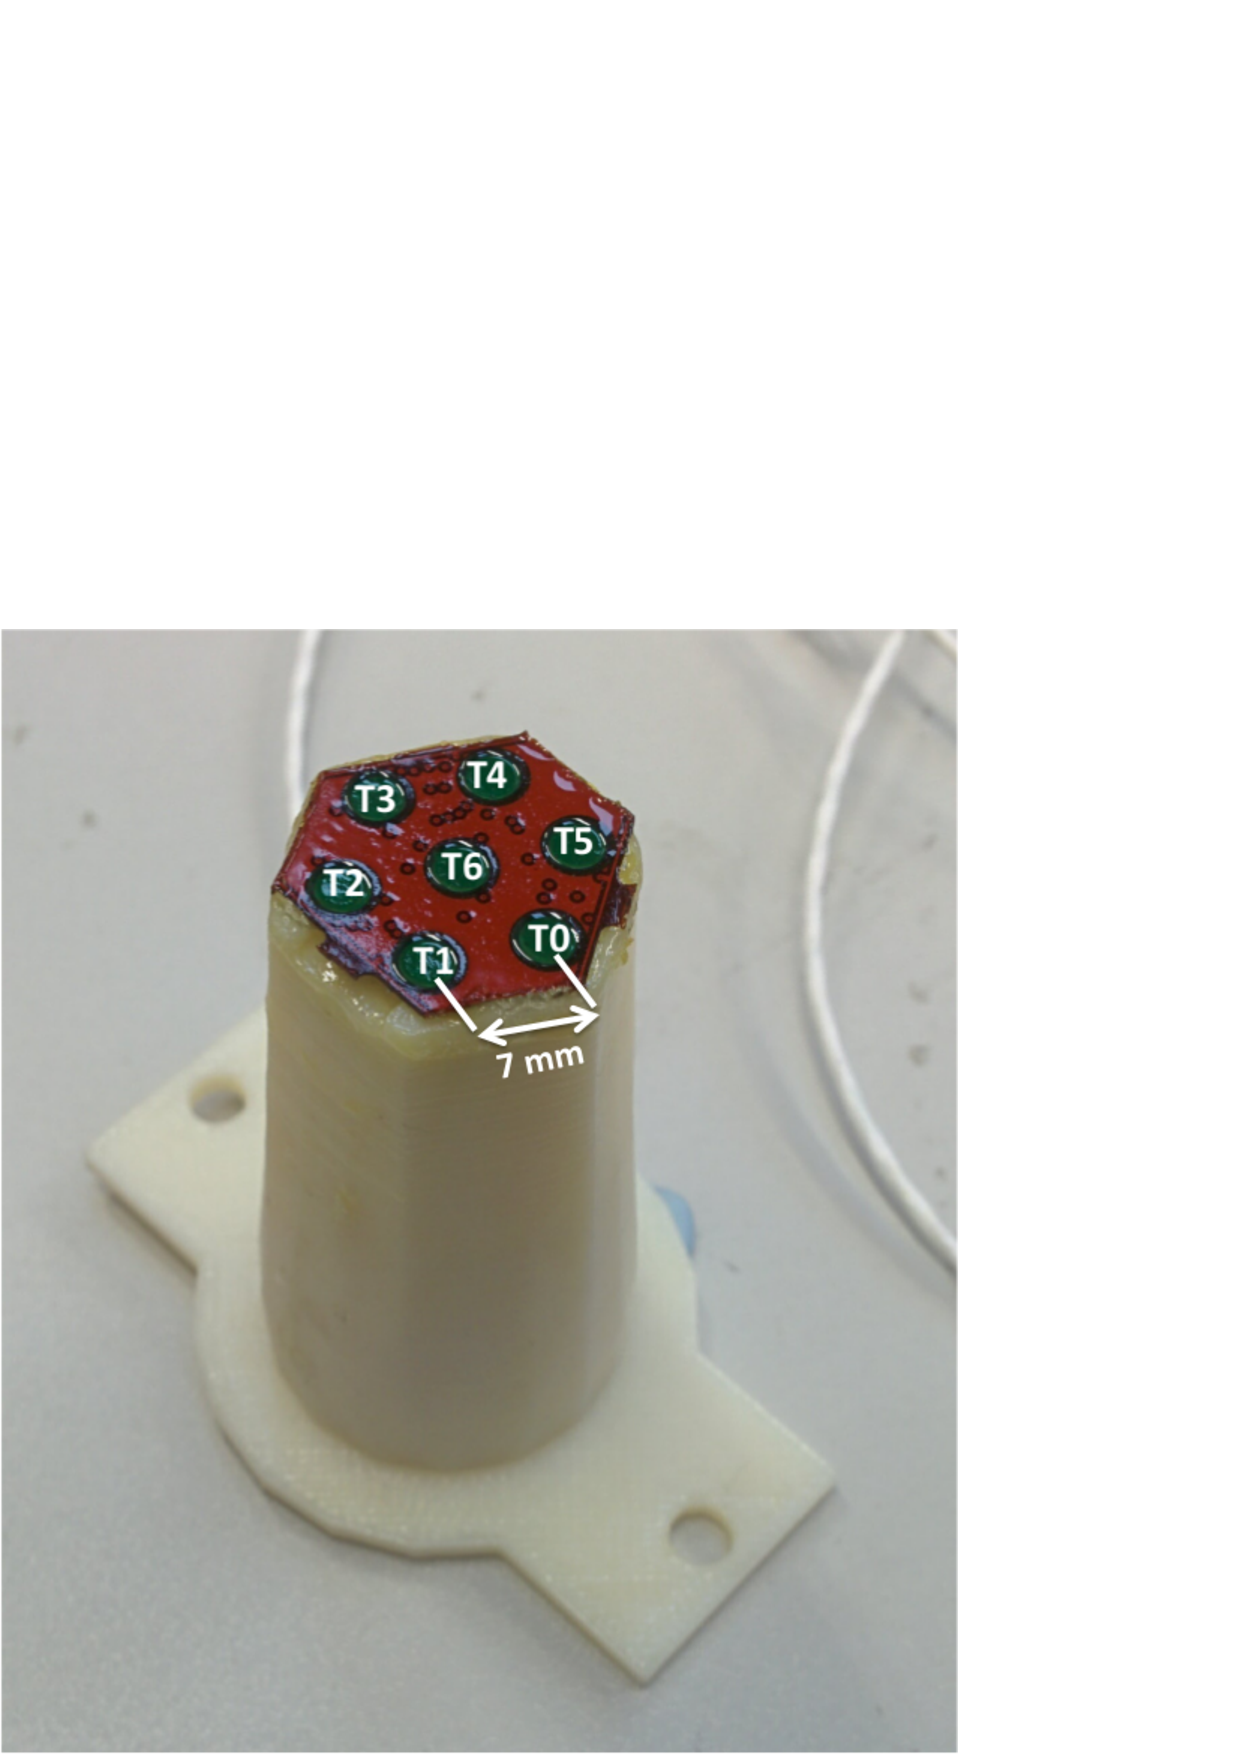
\includegraphics[width=\textwidth]{./figs/probefreccia.pdf}
		\caption{}
		\label{exp:probe}
	\end{subfigure}
	\caption{(a) The CySkin technology architecture. The hexagonal patch is connected to a Intelligent Hub Board (IHB) that collect the tactile sensor data and send them to the PC through a CAN bus. (b) The CySkin patch used for the experiments. It is composed by 6 interconnected triangular modules, each hosting 10 taxels. (c) The experimental setup used for performing the experiments. (d) The sensorised probe.}
	\label{CySkin}
\end{figure}
\subsection{Autonomous Category Formation}\label{sec_unsup_clustering}


We propose an unsupervised process to automatically cluster tactile sensor readings from probed locations in a phantom into five categories. After acquiring tactile image sequences for each probed location, the autonomous category formation process is mainly divided in two pipelined steps: Principal Component Analysis projection ($PCA$) \cite{tipping_probabilistic_1999} and K-Means Clustering ($KMC$) \cite{lloyd_least_1982}. We use the proposed process to observe the influence motion primitives have on sensory inputs and therefore on category formation.

We start the process with tactile image sequences for each probed location in the phantom. The details of the image sequences capture are irrelevant for the generic process here described, thus we leave their explanation to later sections. For a set of $N$ different locations, let $\mathbf{X}$ be a $(N\times D)$ matrix where each unique tactile image sequence for a probed location is a $D$  dimensional row ($D\gg2$) in the matrix. As previously mentioned, we define a tactile image sequence as a sequence of sensor readings, each of which is sequentially concatenated into a single array. The dimension of $D$, then, will be strictly dependent on the motion primitive and on the space interval at which it is decided to capture each tactile image within the time sequence. After obtaining the tactile image sequences matrix $\mathbf{X}$, we begin the process be finding the average tactile sequence $\vec{\mu}$ as:
\begin{equation}
\vec{\mu} = \frac{1}{n}\sum_{i=1}^{n}\vec{x}_i
\end{equation}
where $\vec{x}_i$ is a column vector corresponding to the $i^{th}$ row in $\mathbf{X}$. We proceed by computing the scatter matrix of $\mathbf{X}$ as
\begin{equation}
\mathbf{S} = \sum_{i=1}^{n}(\vec{x}_i-\vec{\mu})(\vec{x}_i-\vec{\mu})^T
\end{equation}
We use Single Value Decomposition to factorize $\mathbf{S}$ into
\begin{equation}
\mathbf{S} = \mathbf{Q}\mathbf{\Lambda} \mathbf{Q}^{-1}
\end{equation}
\noindent where $\mathbf{Q}$ is matrix such that each column $q_j$ corresponds to an eigenvector of $\mathbf{S}$, and each element $\lambda_{jj}$ in the diagonal matrix $\Lambda$ is its corresponding eigenvalue. 

We list the eigenvectors in ascending order of eigenvalue and select the first two in the list. Let $\vec{p}_1$ and $\vec{p}_2$ be the selected eigenvectors obtained from $PCA$. We form a $(D\times 2)$ projection matrix $\mathbf{P}$ as:
\begin{equation}
\mathbf{P}=\begin{bmatrix}\vec{p}_1^{\ T}, \vec{p}_2^{\ T}\end{bmatrix}	
\end{equation}
where $\vec{p}_1^{\ T}$ and $\vec{p}_2^{\ T}$ are column vectors in $\mathbf{P}$. Finally, we project the $D$-dimensional row vectors in $\mathbf{X}$ onto a 2-dimensional subspace by:
\begin{equation}
\mathbf{W}=\mathbf{X}\cdot \mathbf{P}
\end{equation}
where $\mathbf{W}$ is a $(N\times 2)$ matrix and each row in it is a 2-dimensional $encoding$ of a tactile image sequence for a probed location. We proceed by using $KMC$, with random centroid initialization, to split the sequences in $\mathbf{W}$ into $k$ clusters, thus:
\begin{equation}
\vec{v} = KMC_{k}(\mathbf{W})
\end{equation}
where $\vec{v}$ is an N-dimensional array, $\forall i\in \{1, 2,\ ...\ , N\}$,   $\vec{v}_i\in\{0, ..., k\}$, and $\forall i\ \exists j.\ i\neq j\ \land\ v_i\neq v_j$ (no one cluster can contain all objects). In general $\vec{v}_i=0\ iff$ the $i^{th}$ tactile image belongs to cluster 0, $\vec{v}_i=1\ iff$ the $i^{th}$ tactile image belongs to cluster 1 (Fig. \ref{self_org_processing}) and so forth, thus the $\vec{v}$ vector contains the cluster membership of each probed location in the initial set. To avoid cluster anomalies due to the random centroid initializations we run the K-Means Clustering algorithm three times and discard the clustering attempt if, after convergence, any of the three cluster guesses vectors differs from any other. In this context, the cluster assignments for each probed location is largely dependent on the motion primitive employed. The change in cluster assignment is the main object of analysis in the following sections.
 \begin{figure}[]
 	\centering
 	\includegraphics[width=.9\textwidth]{./figs/motion_primitive_preprocessing.pdf}
 	\caption{Autonomous category formation steps.} %{After acquiring morphologically processed $tactile\ images$ for each object in a set, the high dimensional images are first projected in a 2-dimensional subspace ($PCA$) and finally clustered in an unsupervised manner through the $KMC$ algorithm. After clustering, $v$ is vector containing the cluster membership of each object in the initial set.}%}
 	\label{self_org_processing}
 \end{figure}
\subsection{Palpation Movements}

\subsection{Experimental Setup}

We build a soft phantom organ using Ecoflex 00-10\footnote[2]{https://www.smooth-on.com/products/ecoflex-00-10/} from Smooth-on. The phantom organ contained hard inclusions placed at two different depth $5mm$ and $15mm$, and having two different diameters namely $7mm$ and $20mm$. Hereafter we may refer to a $5mm$ inclusion placed at a depth of $7mm$ as `$ss$', a $15mm$ inclusion placed at $7mm$ as `$bs$', a $5mm$ inclusion placed at $20mm$ as `$sd$' and a $15mm$ inclusion placed at $20mm$ as `$bd$'.
The hard nodules have been designed and printed with a 3D printer.
Figure \ref{phantom} shows the position and dimension of the hard nodules and how 

\begin{figure}[]
	\centering
	\begin{subfigure}[b]{0.48\textwidth}
		\begin{subfigure}[b]{\textwidth}
			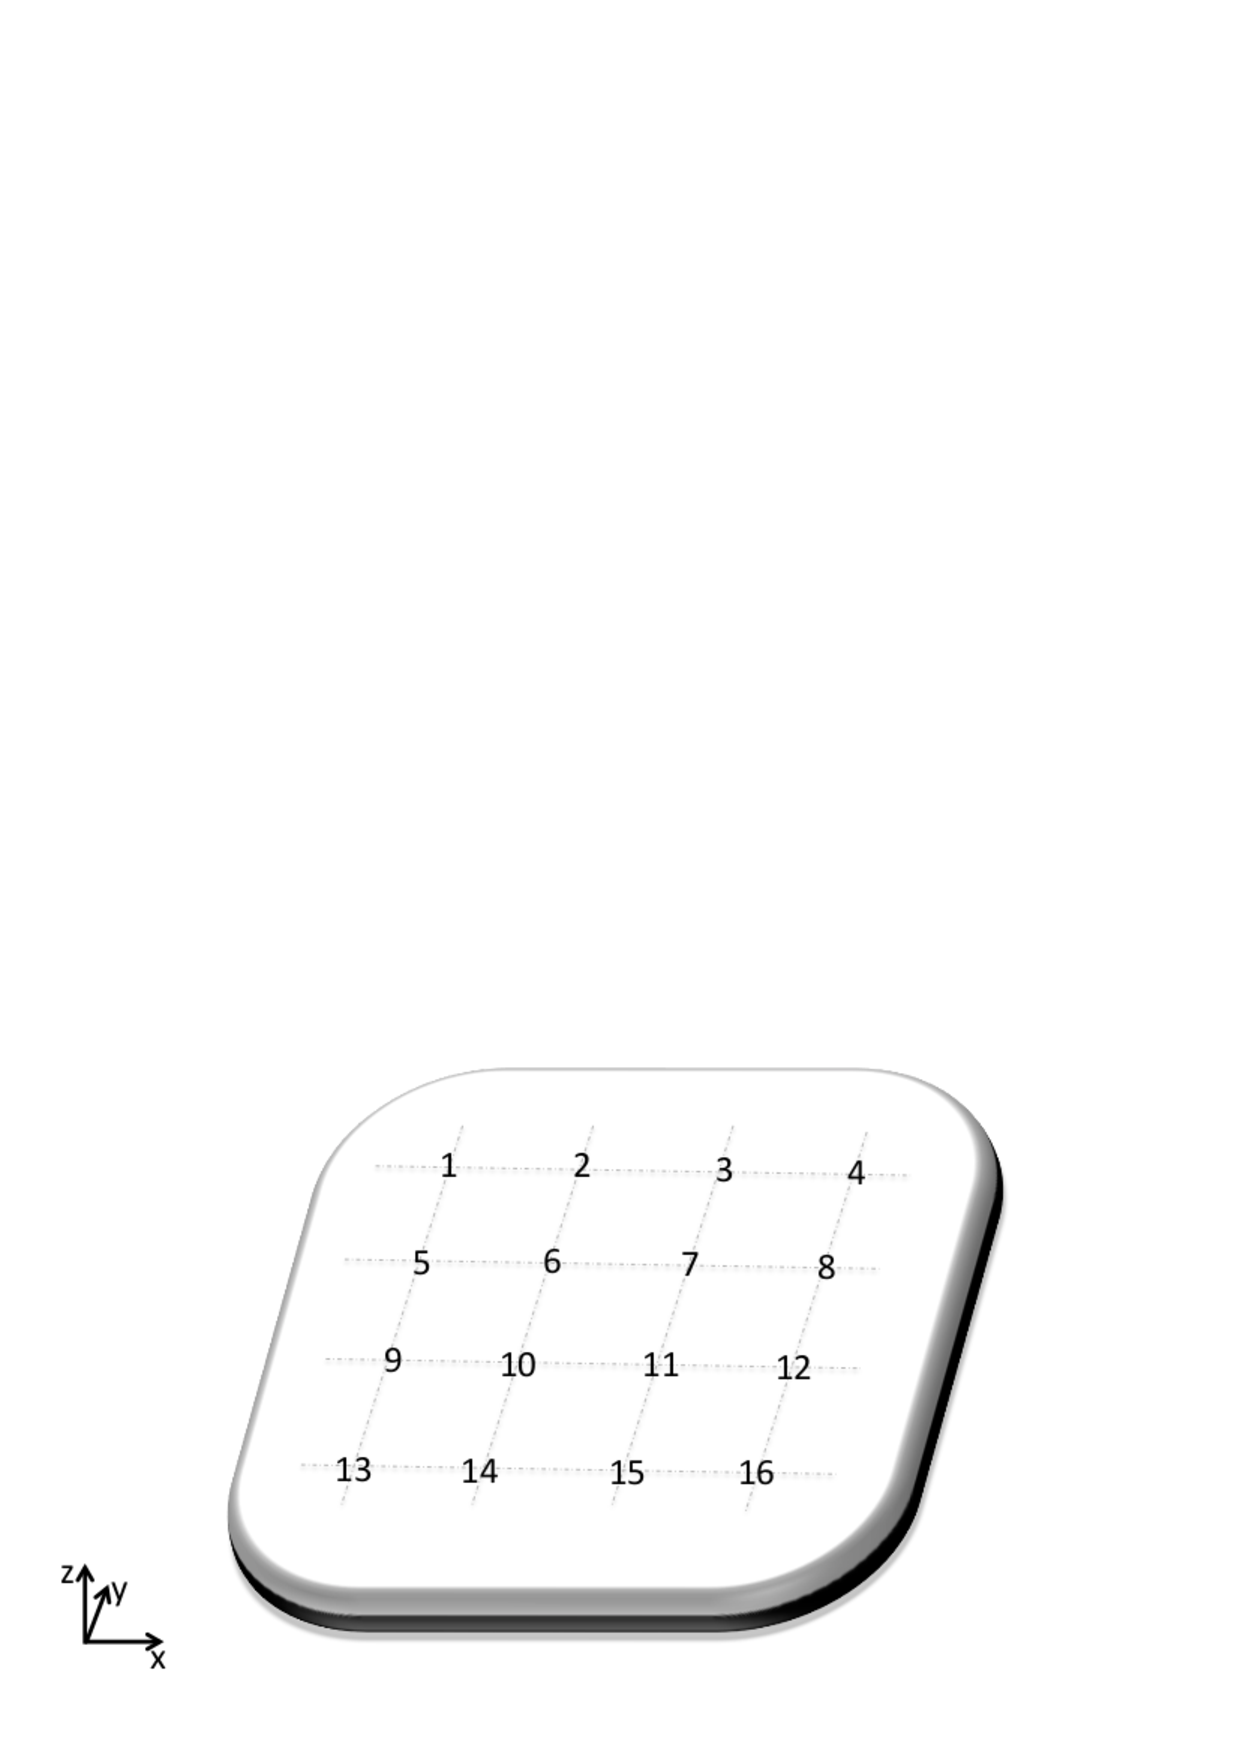
\includegraphics[width=\textwidth]{./figs/phlocations.pdf}
			\caption{}
			\label{phantomgrid:3d}
		\end{subfigure} 
		\vspace{0.025\textwidth}
		\begin{subfigure}[b]{\textwidth}
			\includegraphics[width=\textwidth]{./figs/phsidenew.pdf}
			\caption{}
			\label{phantomgrid:description}
		\end{subfigure}
	\end{subfigure}
	\caption{(a)... (b)... (c)... }
	\label{phantomgrid}
\end{figure}

\begin{figure}[]
	\centering
	\begin{subfigure}[b]{0.48\textwidth}
		\begin{subfigure}[b]{.7\textwidth}
			\includegraphics[width=\textwidth]{./figs/phantom.jpg}
		\end{subfigure} 
		\vspace{0.025\textwidth}
		\begin{subfigure}[b]{.2\textwidth}
			\includegraphics[width=\textwidth]{./figs/table_presence.pdf}
		\end{subfigure}
	\caption{}
	\label{phantom:1}
	\end{subfigure}
	\begin{subfigure}[b]{0.48\textwidth}
		\begin{subfigure}[b]{.7\textwidth}
			\includegraphics[width=\textwidth]{./figs/ph2.jpg}
		\end{subfigure} 
		\vspace{0.025\textwidth}
		\begin{subfigure}[b]{.2\textwidth}
			\includegraphics[width=\textwidth]{./figs/table_presence.pdf}
		\end{subfigure}
	\caption{}
	\label{phantom:2}
	\end{subfigure}
	\caption{(a)... (b)... (c)... }
	\label{phantom}
\end{figure}

%\begin{figure}[]
% 	\centering
% 	\begin{subfigure}[b]{.37\textwidth}
% 		\includegraphics[width=\textwidth]{./figs/phantom.jpg}
% 		\caption{}
% 		\label{phantom:description}
% 	\end{subfigure} 
% 	\hspace{0.01\textwidth}
% 	\begin{subfigure}[b]{0.58\textwidth}
% 		\includegraphics[width=\textwidth]{./figs/phschema.jpg}
% 		\caption{}
% 		\label{phantom:real}
% 	\end{subfigure}
% 	\caption{(a) (b) }
% 	\label{phantom}
% \end{figure}
We 3D-print a custom-made end-effector onto which we integrate a capacitive tactile sensor onto its surface to retrieve $tactile\ images$ during the probing experiments.

 


We carry out the experiments by mounting the printed end-effector, coupled with the tactile sensor, onto an ST-Robotics R12/5 robotic arm\footnote[3]{http://www.robotshop.com/uk/st-robotics-r12-5-axis-articulated-robot-arm.html}.  (Fig. \ref{setup}). 
%We place a FlexiForce force sensor\footnote[4]{https://www.tekscan.com/products-solutions/force-sensors/a502} at the base of the object in order to record the perpendicular force exerted during the probing motions.  








\subsection{Experimental protocol} \label{sec_experimental_protocol}

%To further remove experimental bias, we repeat each set of experiments three times and average the computed $tactile\ images$ over the three trials. We finally construct the tactile image matrix $\mathbf{X}$ by setting each of its rows to a computed tactile image.
%
%
%We utilize the process described in Section \ref{sec_unsup_clustering} to process the tactile image matrix for each experiment. 
%
%The unsupervised part of the process (PCA \& KMC) clusters the tactile data automatically based on the two dimensions of highest variance in the data. We define the cluster matching process $\mathbf{CM}$ as:
%\begin{equation}
%\vec{v}^{\ \prime} = \mathbf{CM}(\vec{v},\ \vec{t})
%\end{equation}

The probing procedure begins with the user teaching the robot the location of the nodules. This is done by manually moving the head to each of the sixteen test locations, taking care to carefully align the head above the centre of each nodule. Once this is done, the robot automatically probes each location in turn using the two motions shown in Figure \ref{probing}. First, the vertical motion is performed, where the probe is aligned vertically and plunged directly down in to the phantom in 0.5 mm increments. After each increment, the robot briefly pauses to allow a tactile image to be recorded before continuing with the next movement. This continues until the probe is at a depth of 20 mm below the surface of the silicone, whereupon it returns to a neutral position 10 mm above the surface in a single movement.

After this, the more complicated rotary probing takes place. During this motion, the robot rotates about a point $d$ mm below the surface of the silicone, keeping the sensor $r$ mm away from this nexus point. First, the robot moves vertically down so that it is at the correct distance from the nexus. It then rotates in the $+\theta$ direction until it is at an radius of 30\degree to the vertical. From here, the probe rotates in the $-\theta$ direction in 1\degree increments, recording a tactile image after each step. Once the probe has moved through 60\degree it stops recording, rotates back to vertical then returns to the neutral position 10 mm above the surface of the silicone. This procedure is repeated for $r\in\lbrace 10 mm, 12 mm, 14 mm, 16 mm \rbrace$ and $d\in\lbrace 10 mm, 12 mm, 14 mm, 16 mm \rbrace$.

\begin{figure}[]
	\centering
	\begin{subfigure}[b]{0.64\textwidth}
		\includegraphics[width=\textwidth]{./figs/motion_diagram}
		\caption{Rotary probing.}
		\label{probing:rotate}
	\end{subfigure}
	\caption{The two probing motions employed.}
	\label{probing}
\end{figure}



\section{Results} \label{sec_results}

After obtaining time series data from the two motion strategies we can finally form the $\mathbf{X}$ tactile image sequence matrix described in Section \ref{sec_unsup_clustering}, and proceed with the Autonomous Category Formation process. At the end of the process, we obtain a $\vec{v}$ vector containing the cluster membership of each probed location in the phantom. To assess the performance of the unsupervised clustering method we first need to match the clusters to the true target classes for the phantom under analysis. We use a cluster matching process based on maximal accuracy i.e.:
\begin{equation}
\vec{v}^{\ \prime} = \mathbf{CM}(\vec{v},\ \vec{t})
\end{equation}
Given the targets $\vec{t}$ and a cluster guess vector $\vec{v}$ then, $\vec{v}\ '$ is a new vector such that 
\begin{flalign*}
&\forall i \in \{1,2, ... , N\}.\\
&\  (\vec{v}_i =1 \implies \vec{v}_i^{\ \prime}=0) \land  (\vec{v}_i =0 \implies \vec{v}_i^{\ \prime}=1)\\
&\iff\ ||\vec{v}-\vec{t}||>||\vec{v}_i^{\ \prime}-\vec{t}||
\end{flalign*} 
Essentially, we associate a cluster guess to a target cluster maximizing accuracy for the particular task (Fig. \ref{cluster_matching}). A vector $\vec{v}=[0\ 0\ 0\ 1]$ for a task $\vec{t}_k=[1\ 1\ 1\ 0]$, for example, would be re-associated as $\vec{v}^{\ \prime}=[1\ 1\ 1\ 0]$. We utilize this to benchmark the performance of the algorithm after palpation.  


\subsection{Presence/Absence of the Nodule}
%We feed the data gathered during experiments to the Unsupervised Clustering process described in Section \ref{sec_unsup_clustering}. 
After matching the clusters emerged to the targets for each probed location, it is possible to interpret the performance of the unsupervised inference given the motion primitive. 

For each probing motion we make a plot of the two dimensional projected tactile image sequences relative to the probing areas in the phantom, and observe how their relative positions within each plot, and thus their two dimensional encodings, changes according to the motion strategy. We initially focus on the vertical motion primitive, and compare the relative position of the probed areas with respect to each other when changing the probing depth.

Figure \ref{ResVertRaw} shows the plots of the raw data as obtained after vertically probing the soft phantom with at a depth of $0.5mm$ and $18.5mm$, respectively the smallest and largest depths explored. Figure \ref{ResVert:dn0} and \ref{ResVert:dn9} shows the corresponding plots of the projected 2D points for each probed location, as computed after PCA, and their resulting classification due to the unsupervised clustering process. From Fig. \ref{ResVert:dn0} and \ref{ResVert:dn9} it is clear how increasing the probing depth improved the clustering accuracy of the algorithm. When probing at a depth of $0.5mm$ (Fig. \ref{ResVert:dn0}) only the large and superficial bead is detectable by the capacitive sensor response. For the areas with the remaining inclusions the retrieved information is so similar to areas where no beads are touched, that the clustering naturally clustered them as empty. However, when probing at a higher depth, the information relative to the big but deep inclusion becomes increasingly closer to that of the big and superficial bead, and is finally clustered as such. The beneficial effect of higher probing depth is also demonstrated by the change in position of small and superficial inclusion ($ss$) from Figure \ref{ResVert:dn0} to Figure \ref{ResVert:dn9},  which, while misclassified, likewise moves closer to the area classified as containing an inclusion. The sensor signal for the small and deep inclusion instead, is perceived as more similar to areas with no bead, as expected intuitively. At higher probing depths, the higher pressure exercised by the finger activates the taxels on or near the area of the bead with higher strength, effectively changing the sensor response to one where the beads are sensed, and allowing the sensor better capture inclusion presence.
%
%\begin{figure}[]
%	\centering
%	\begin{subfigure}[b]{.48\textwidth}
%		\includegraphics[width=\textwidth]{./figs/phantom2propertiesVertical_accuracy_.jpg}
%		\caption{}
%		\label{ResVertAccMetrics:acc}
%	\end{subfigure}
%	\begin{subfigure}[b]{.48\textwidth}
%		\includegraphics[width=\textwidth]{./figs/phantom2propertiesVertical_silhouette.jpg}
%		\caption{}
%		\label{ResVertAccMetrics:silhouette_score}
%	\end{subfigure}
%	\caption{Figure (a) and (b) show respectively the accuracy and the silhouette score of the emerged categories when varying the depth parameter (see Section \ref{sec_experimental_protocol}).}
%	\label{ResVertAccMetrics}
%\end{figure}

\begin{minipage}{\textwidth}
	\begin{figure}[H]
		\centering
		\begin{subfigure}[b]{.9\textwidth}
			\centering
			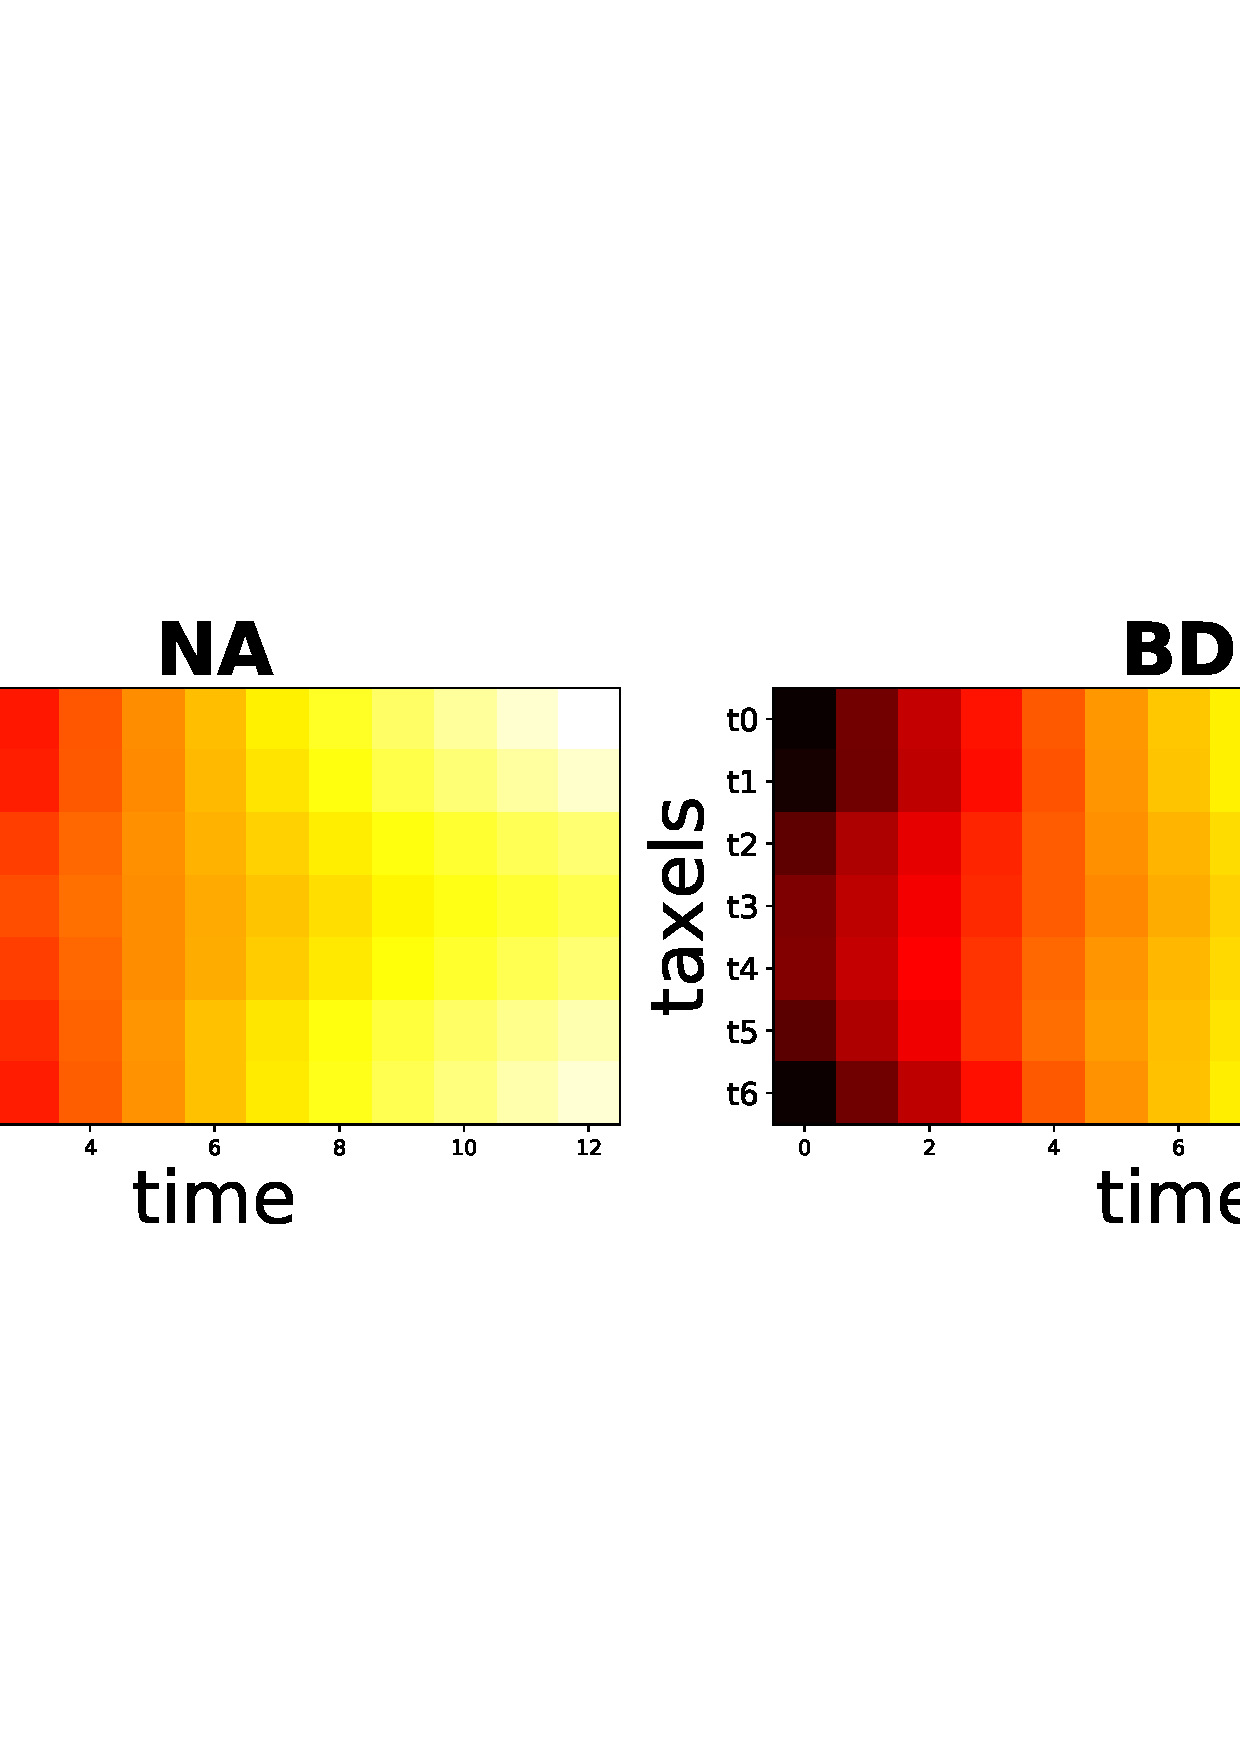
\includegraphics[width=\textwidth]{./figs/phantom2properties_rawdataf_Vertical-d14_5.jpg}
			\caption{Raw Data Samples}
			\label{Raw:v1}
			\vspace{8pt}
		\end{subfigure} 
		\caption{Figure (a) and (b) show the raw data sensor response when probing the first and second soft phantom respectively in an area containing an inclusion $15mm$ in diameter placed at $20mm$ ($bd$) through a vertical motion primitive. Figure (c) and (d) show the raw data sensor response when probing the phantoms in a location containing a $bd$ inclusion, through the rotatory motion primitive.
		}
		\label{Raw}
	\end{figure}
	
	\begin{figure}[H]
		\centering
		\hspace{0.03\textwidth}
		\begin{subfigure}[b]{.45\textwidth}
			\includegraphics[width=\textwidth]{./figs/phantom2properties_pcafig_Vertical-d14_5.jpg}
			\caption{}
			\label{hist:1}
		\end{subfigure}
		\begin{subfigure}[b]{.45\textwidth}
			\includegraphics[width=\textwidth]{./figs/phantom2properties3-12-13-21-42-24-31-31-2_pcafig_Rotate-d190-r120.jpg}
			\caption{}
			\label{hist:2}
		\end{subfigure}
		\caption{The figures show the explained variance of each principal component, when computed for the PCA projection, in two different scenario. In the first (a) the phantom is probed with a vertical motion at a depth of $d=14.5mm$ while in the second (b) the probe is probed with a rotatory motion, where $d=19mm$ and $r=12mm$, using only 8 samples from the phantom. As clear from the Figure, the motion and the sample number directly affects the explained variance, as through them we can effect the amount by which the first components explain the variance of the data.}
		\label{hist}
	\end{figure}
	
	\begin{figure}[H]
		\centering
		\begin{subfigure}[b]{0.48\textwidth}
			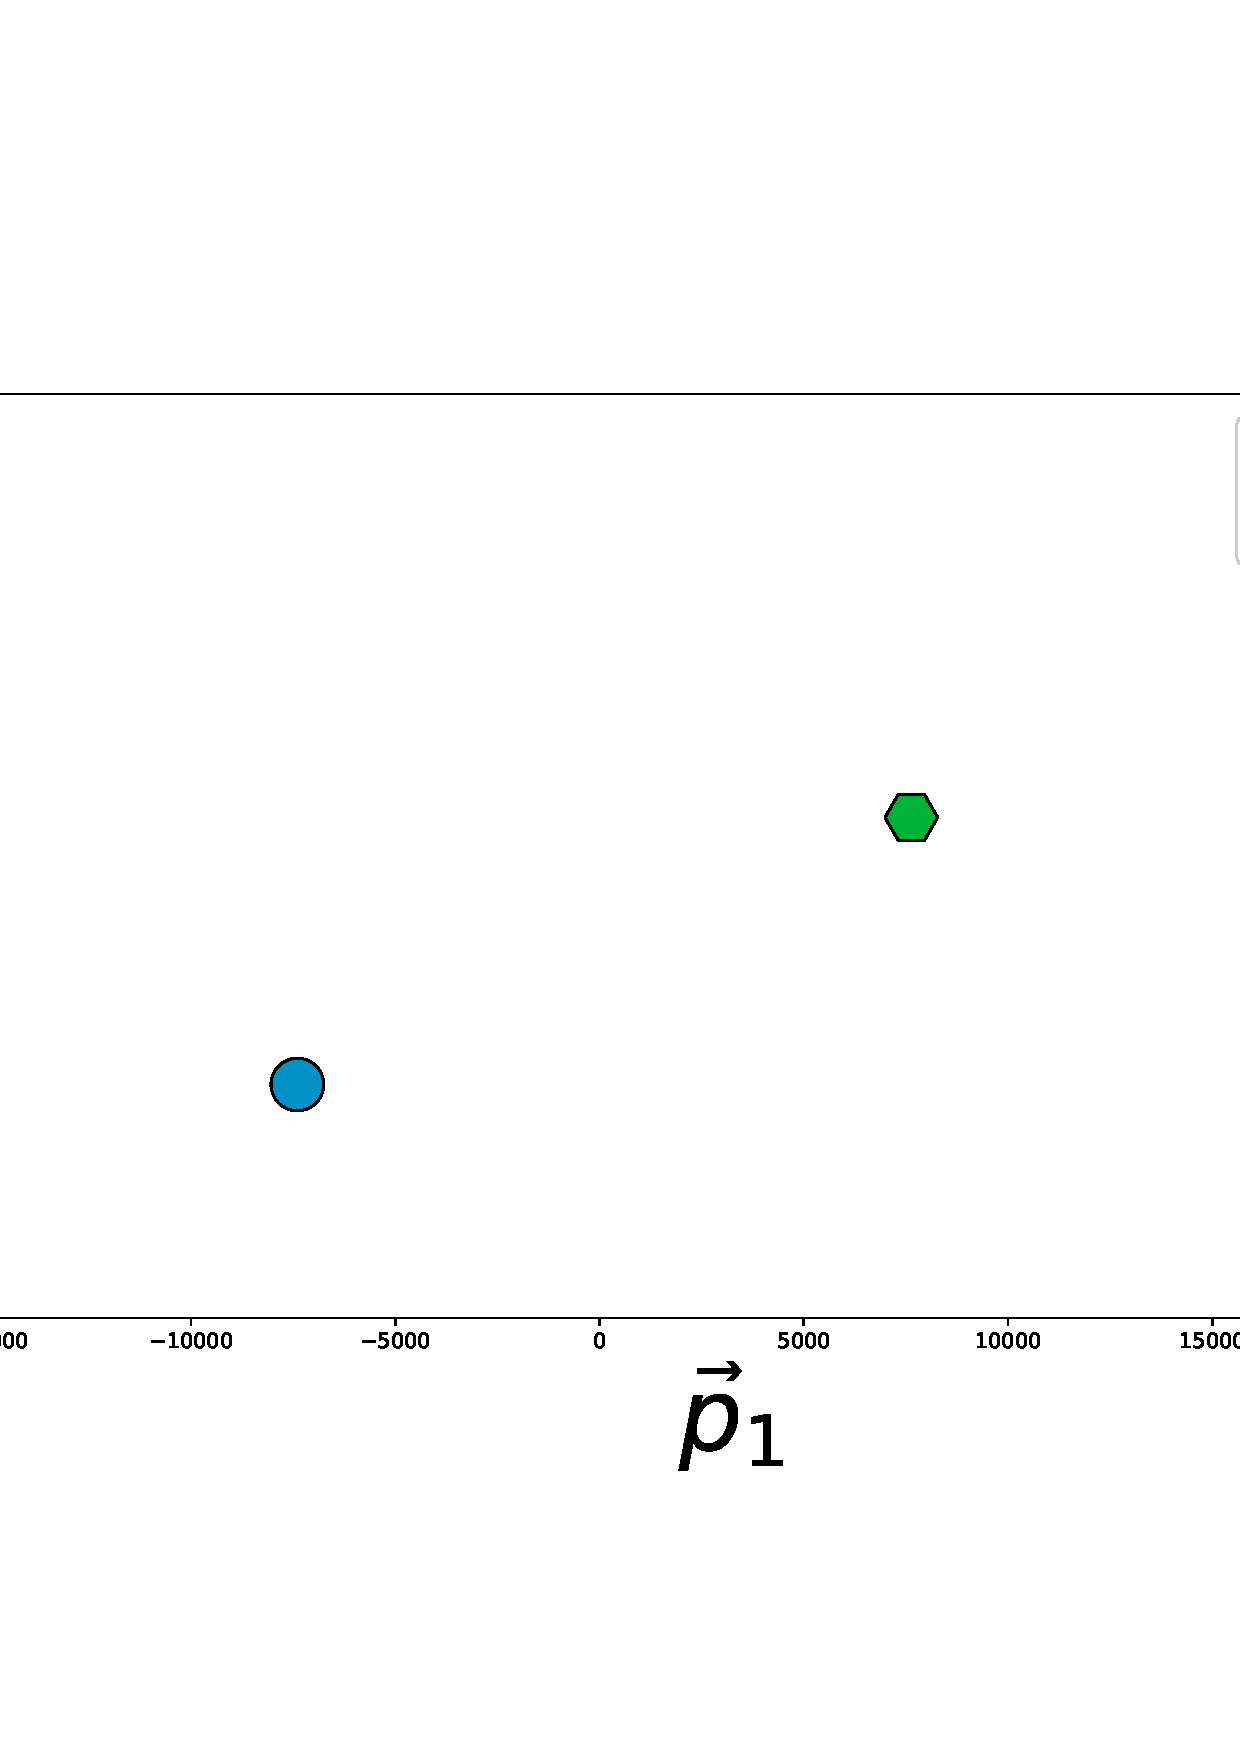
\includegraphics[width=\textwidth]{./figs/phantom2properties_nabdfig_Vertical-d14_5.jpg}
			\caption{PCA Projected Samples}
			\label{Raw:v2}
		\end{subfigure}
		
	\end{figure}
	\hfill\\
\end{minipage}


We asses the clustering performance of the process for each varying depth through two metrics: accuracy and silhouette score. The accuracy is computed by simply retrieving the proportion of correctly classified elements in $\vec{v}'$ with respect to the targets $\vec{t}$. The silhouette score (REFERENCE), is a number $\in [-1,1]$ and provides a measure of the quality of the clusters obtained for each probing and is based on both the intra-cluster distance of each cluster and the mean nearest-cluster distance for each sample. Figure \ref{ResVertAccMetrics} shows the values for both metrics when varying the depth of probing. As clear from the figure, we find the optimal probing motion to be the at the maximal explored depth.

%\NoteP{Let's wait for conf matries here.. can't show any difference}
%Figure FIGURE shows the confusion matrices of the cluster guesses with respect to the true state of the probed area.
%\begin{figure}[]
%	\centering
%	\begin{subfigure}[b]{.35\textwidth}
%		\includegraphics[width=\textwidth]{./figs/properties_cm_Vertical-dn0-NA.jpg}
%		\caption{}
%		\label{Resvertcm:dn0}
%	\end{subfigure} 
%	\hspace{0.01\textwidth}
%	\begin{subfigure}[b]{0.35\textwidth}
%		\includegraphics[width=\textwidth]{./figs/properties_cm_Vertical-dn6-NA.jpg}
%		\caption{}
%		\label{Resvertcm:dn9}
%	\end{subfigure}  
%	\caption{Confusion matrices corresponding to the clustering results obtained with different parameters for the vertical movement. The diagonal in each matrix retains the counts for the correct cluster guesses.}
%	\label{Resvertcm}
%\end{figure}

After Vertical motion, we test the effects of both radius and radius of rotation of the rotary motion primitive. Similarly to the earlier analysis, we wish to see how the relative position of the sensed probed areas changes according to the change in motion strategy (Fig. \ref{ResRot}).  Fig. \ref{ResFeatRot:100-100} shows the clustering emerged when using a rotatory motion primitive with the smallest tested rotation and depth. As clear from the figure the response of the sensor when touching all beads, except for one that's both large and in the surface ($bs$), is very similar to the response obtained when probing areas with no bead. As the rotation of motion increases, the classification  improves and the large bead is correctly classified even when deep in the phantom (Fig. \ref{ResFeatRot:100-160}). The increase in depth, similarly, improves classification by changing the sensory response for the large-deep bead into one closer to a strong bead presence response. More interestingly, however, is the change in intra-cluster distance observed for the areas where no bead was observed (blue positions from Fig. \ref{ResFeatRot:100-100} to Fig. \ref{ResFeatRot:160-100}). The result suggests that a consequence of increasing the depth of motion is also an increase in certainty of how an $empty$ area should look like. Ultimately, the combination of the increase in the two motion primitive parameters increases accuracy further, allowing the pre-processed sensory input to be discriminative enough to recognize small beads when these are close to the surface of the phantom (Fig. \ref{ResFeatRot:160-160}). Moreover, the intra-cluster variance for the nodule absence cluster does not change significantly from the only previous case (Fig. \ref{ResFeatRot:160-100}) suggesting that rotation, if helpful in sensing nodules when these are present, does not significantly change the sensor response when the probed location is empty. The two parameters, then, have a complementary rather than conflicting relation to each other for the task as hand. 


\begin{minipage}{\textwidth}
	\begin{figure}[H]
		\centering
		\begin{subfigure}[b]{.48\textwidth}
			\includegraphics[width=\textwidth]{./figs/Vertical_explained_variance_quantity.jpg}
			\caption{Vertical Motion}
			\label{inf_retention_quantity:vertical}
		\end{subfigure}
		\begin{subfigure}[b]{.48\textwidth}
			\includegraphics[width=\textwidth]{./figs/Rotation_explained_variance_quantity.jpg}
			\caption{Rotatory Motion}
			\label{inf_retention_quantity:Rotation}
		\end{subfigure}
		\caption{The figure show the change in explained variance by the 2D PCA subspace projection, when proving Vertically (a) and through the rotatory motion (b), changing the number of samples used to find the principal components ($N$ in $\mathbf{X}$, see Section \ref{sec_unsup_clustering}). }
		\label{inf_retention_quantity}
	\end{figure}
	\begin{figure}[H]
		\centering
		\begin{subfigure}[b]{.48\textwidth}
			\includegraphics[width=\textwidth]{./figs/Vertical_explained_variance_quality.jpg}
			\caption{Vertical Motion}
			\label{inf_retention_quality:vertical}
		\end{subfigure}
		\begin{subfigure}[b]{.48\textwidth}
			\includegraphics[width=\textwidth]{./figs/Rotation_explained_variance_quality.jpg}
			\caption{Rotatory Motion}
			\label{inf_retention_quality:Rotation}
		\end{subfigure}
		\caption{The figure show the change in explained variance by the 2D PCA subspace projection, when proving Vertically (a) and through the rotatory motion (b), changing the quality of the samples used to find the principal components, while maintaining their number constant. }
		\label{inf_retention_quality}
	\end{figure}
\hfill\\
\end{minipage}


\begin{minipage}{\textwidth}
	\begin{figure}[H]
		\centering
		\begin{subfigure}[b]{.43\textwidth}
			\includegraphics[width=\textwidth]{./figs/nabd_rawdataf_Vertical-d6_5.jpg}
			\caption{Vertical Motion: $depth=6.5mm$}
			\label{rawnabs:d6_5}
		\end{subfigure}
		\hspace{0.02\textwidth}
		\begin{subfigure}[b]{.43\textwidth}
			\includegraphics[width=\textwidth]{./figs/nabd_rawdataf_Vertical-d19_5.jpg}
			\caption{Vertical Motion: $depth=19.5mm$}
			\label{rawnabs:d19_5}
		\end{subfigure}
		\caption{Raw NA-BS in na-bs cluster}
		\label{rawnabs}
	\end{figure}
	\begin{figure}[H]
		\centering
		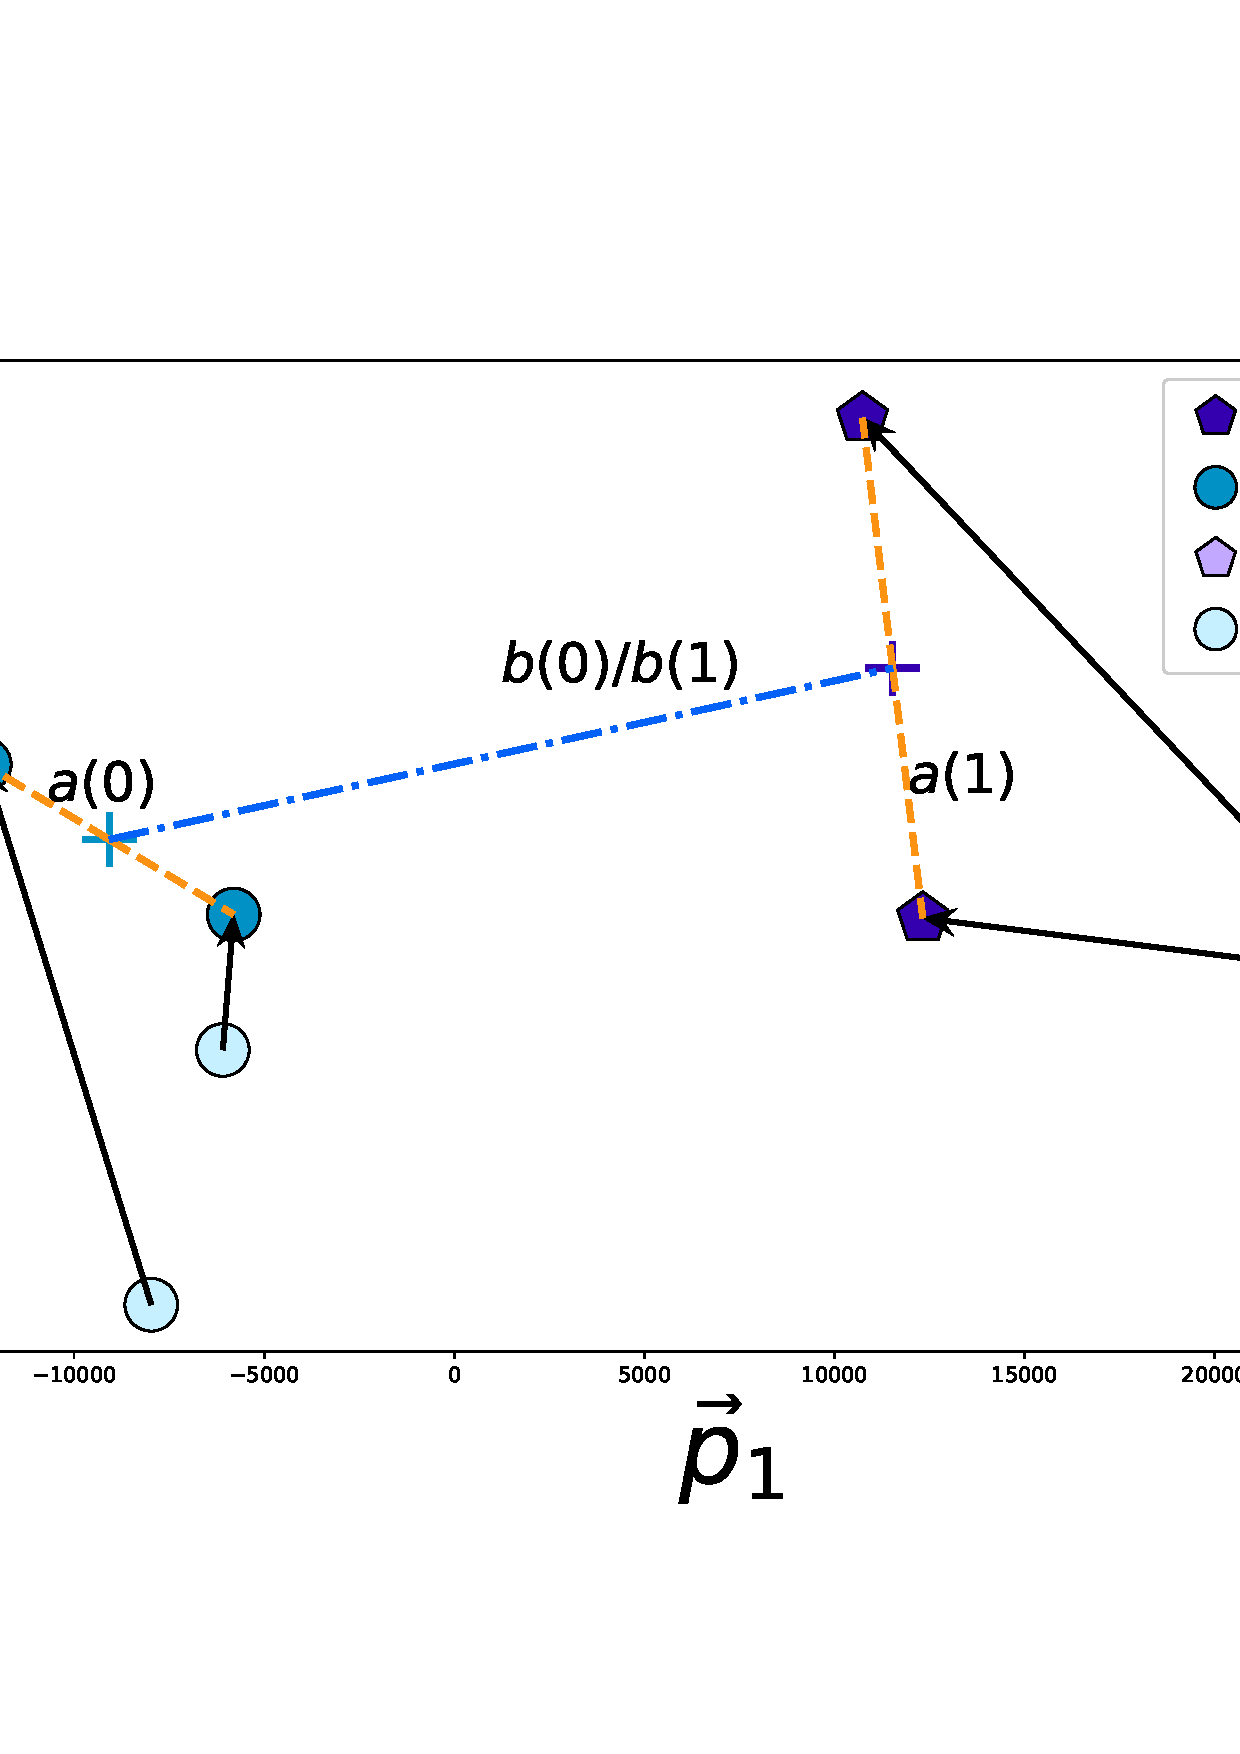
\includegraphics[width=.8\textwidth]{./figs/flow.jpg}\hspace{0.07\textwidth}
		\caption{NA and BD motion when going from a vertical probing depth of $6.5mm$ to a depth of $19.5mm$.}
		\label{flow}
	\end{figure}
\hfill\\
\end{minipage}




\begin{figure}[]
	\centering
	\begin{subfigure}[b]{\textwidth}
		\begin{subfigure}[b]{.48\textwidth}
			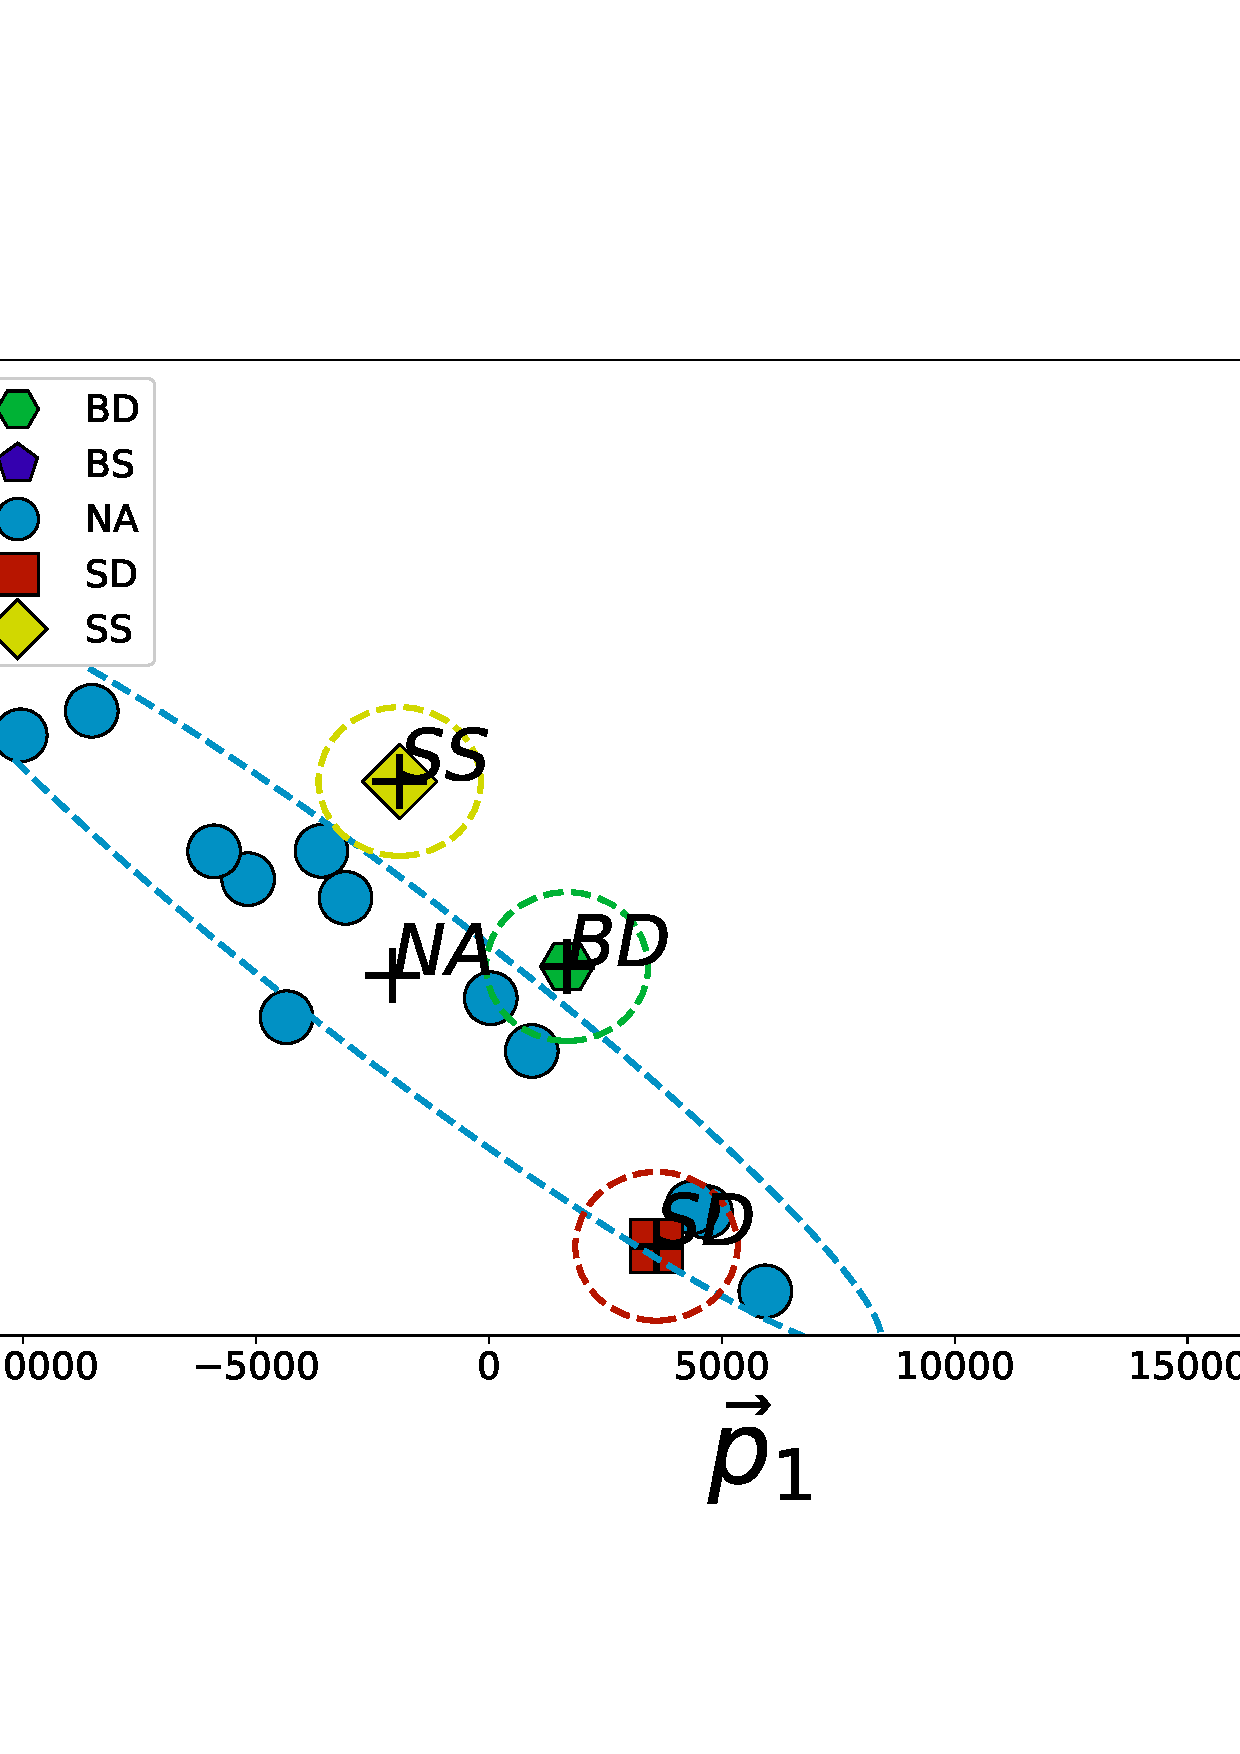
\includegraphics[width=\textwidth]{./figs/phantom1properties_clsplt_Vertical-d6_5.jpg}
			\caption{\tiny{Vertical: $depth=0.5mm$}}
			\label{ResVert:dn0}
		\end{subfigure} 
		\hspace{0.01\textwidth}
		\begin{subfigure}[b]{0.48\textwidth}
			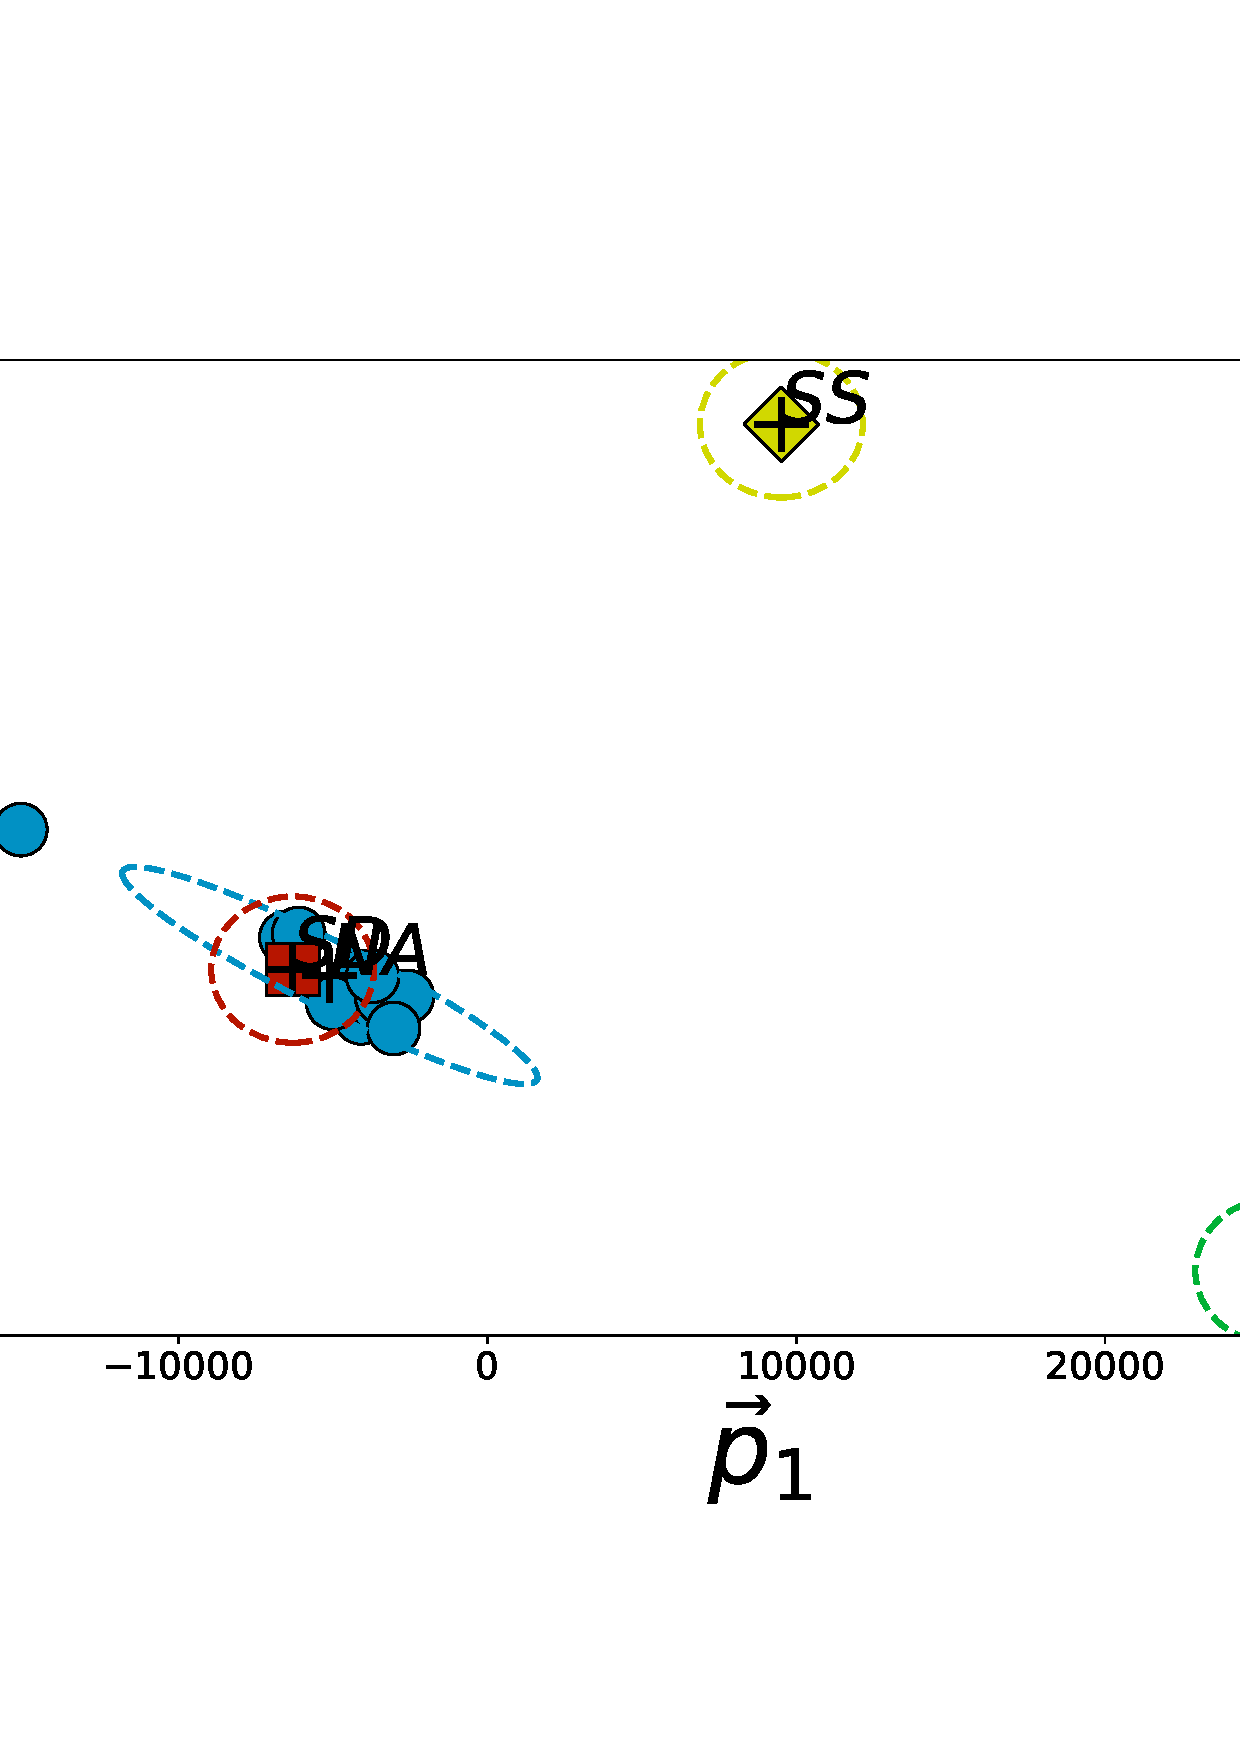
\includegraphics[width=\textwidth]{./figs/phantom1properties_clsplt_Vertical-d19_5.jpg}
			\caption{\tiny{Vertical: $depth=18.5mm$}}
			\label{ResVert:dn9}
		\end{subfigure}
	\vspace{20pt}
	\end{subfigure}
	\begin{subfigure}[b]{\textwidth}
		\begin{subfigure}[b]{.48\textwidth}
			\includegraphics[width=\textwidth]{./figs/phantom1properties_clsplt_Rotate-d100-r100.jpg}
			\caption{\tiny{Rotatory: $depth=10mm$, $radius=10m$}}
			\label{ResRot:100-100}
		\end{subfigure} 
		\hspace{0.01\textwidth}
		\begin{subfigure}[b]{0.48\textwidth}
			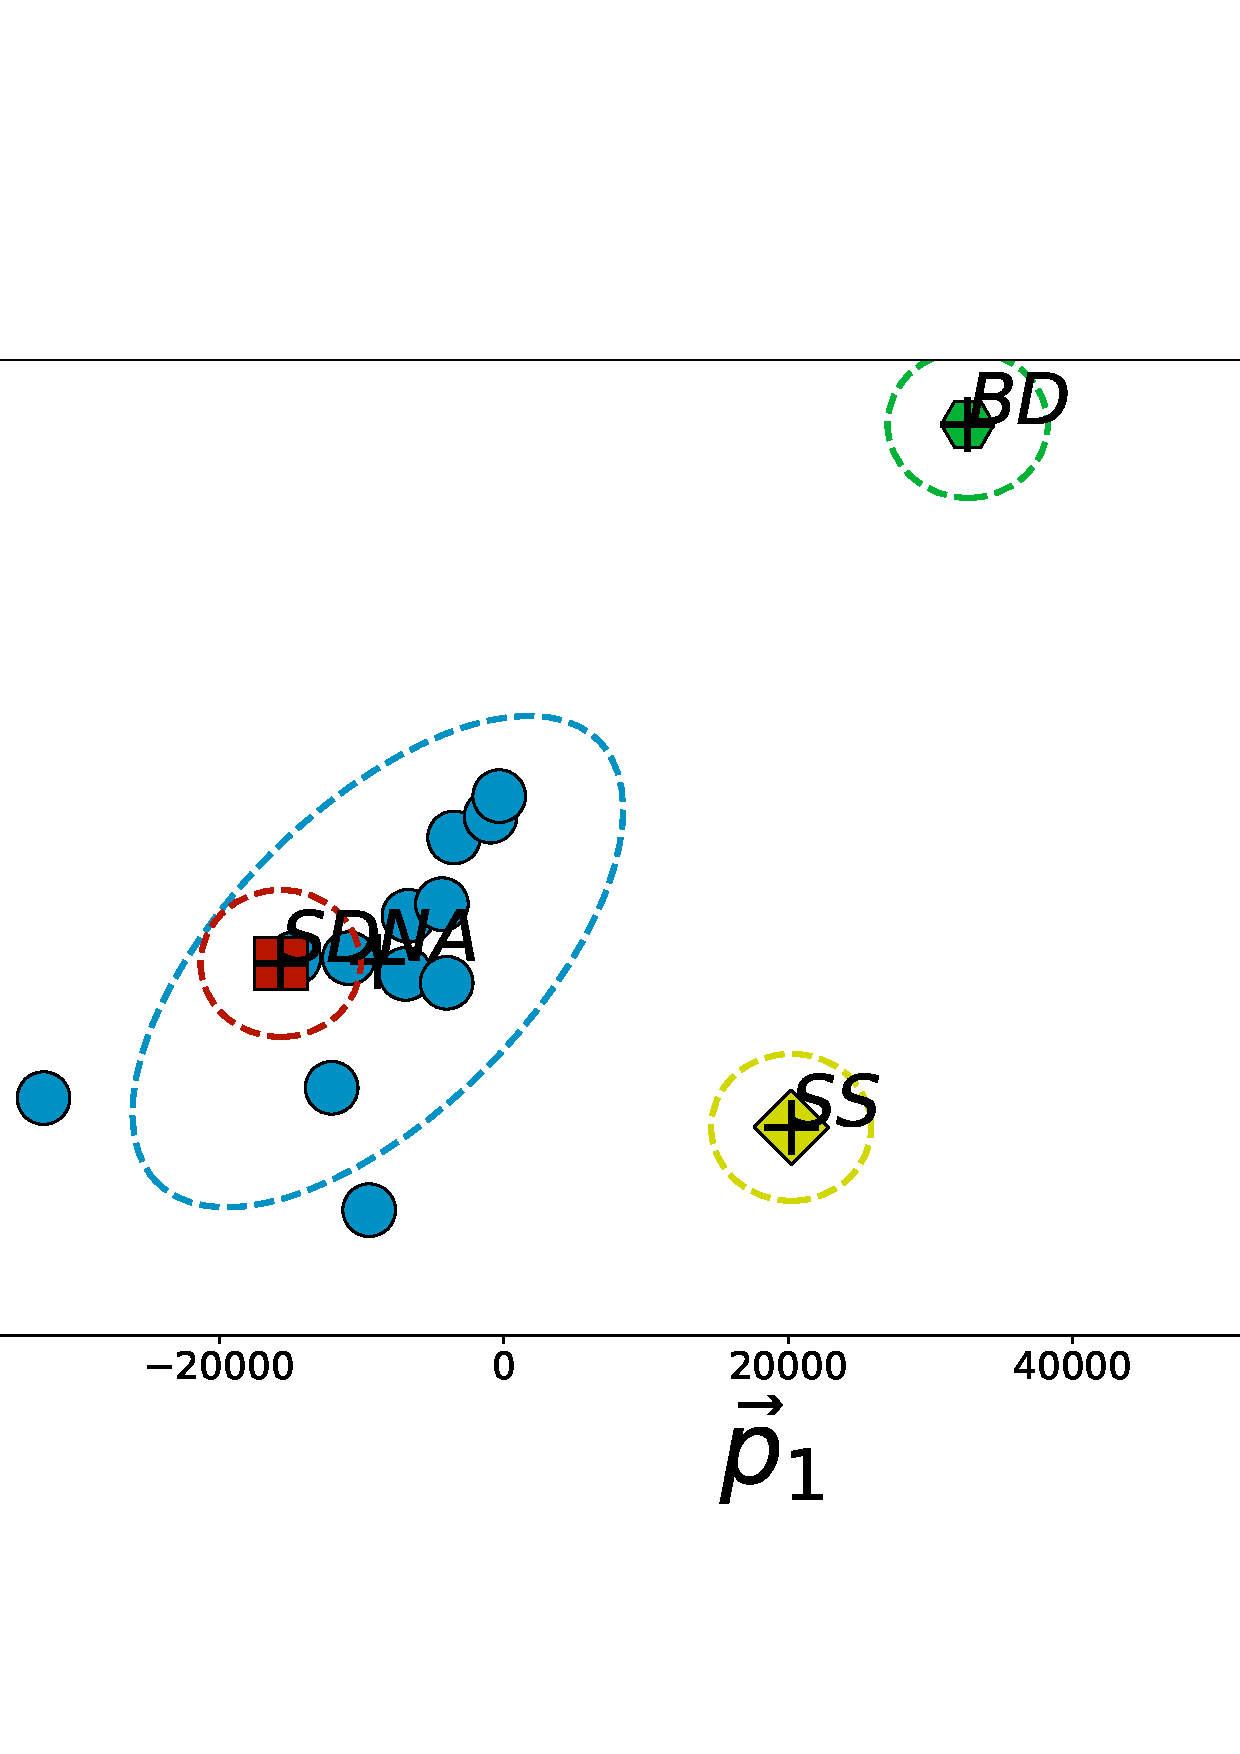
\includegraphics[width=\textwidth]{./figs/phantom1properties_clsplt_Rotate-d100-r160.jpg}
			\caption{\tiny{Rotatory: $depth=10mm$, $radius=16mm$}}
			\label{ResRot:100-160}
		\end{subfigure}
	\vspace{4pt}
	\end{subfigure}
	\begin{subfigure}[b]{\textwidth}
		\begin{subfigure}[b]{0.48\textwidth}
			\includegraphics[width=\textwidth]{./figs/phantom1properties_clsplt_Rotate-d160-r100.jpg}
			\caption{\tiny{Rotatory: $depth=16mm$, $radius=10mm$}}
			\label{ResRot:160-100}
		\end{subfigure}
		\hspace{0.01\textwidth}
		\begin{subfigure}[b]{0.48\textwidth}
			\includegraphics[width=\textwidth]{./figs/phantom1properties_clsplt_Rotate-d160-r160.jpg}
			\caption{\tiny{Rotatory: $depth=16mm$, $radius=16mm$}}
			\label{ResRot:160-160}
		\end{subfigure}
	\end{subfigure}
	\caption{The Figure shows the 2-dimensional projection
	of different combination of depth and radius on the two axis of highest variance in the
	data for rotational movement (a) depth = 10, radius = 10 deg (b) depth = 10, radius = 16 deg (c) depth = 16, radius = 10 (d) depth = 16, radius - 16. The line $l_{kmc}$ corresponds to the decision boundary of the two cluster as found by the KMC algorithm, and C0 and C1 their corresponding centroids.}
\end{figure}



\begin{minipage}{\textwidth}
	\begin{figure}[H]
		\centering
		\begin{subfigure}[b]{.48\textwidth}
			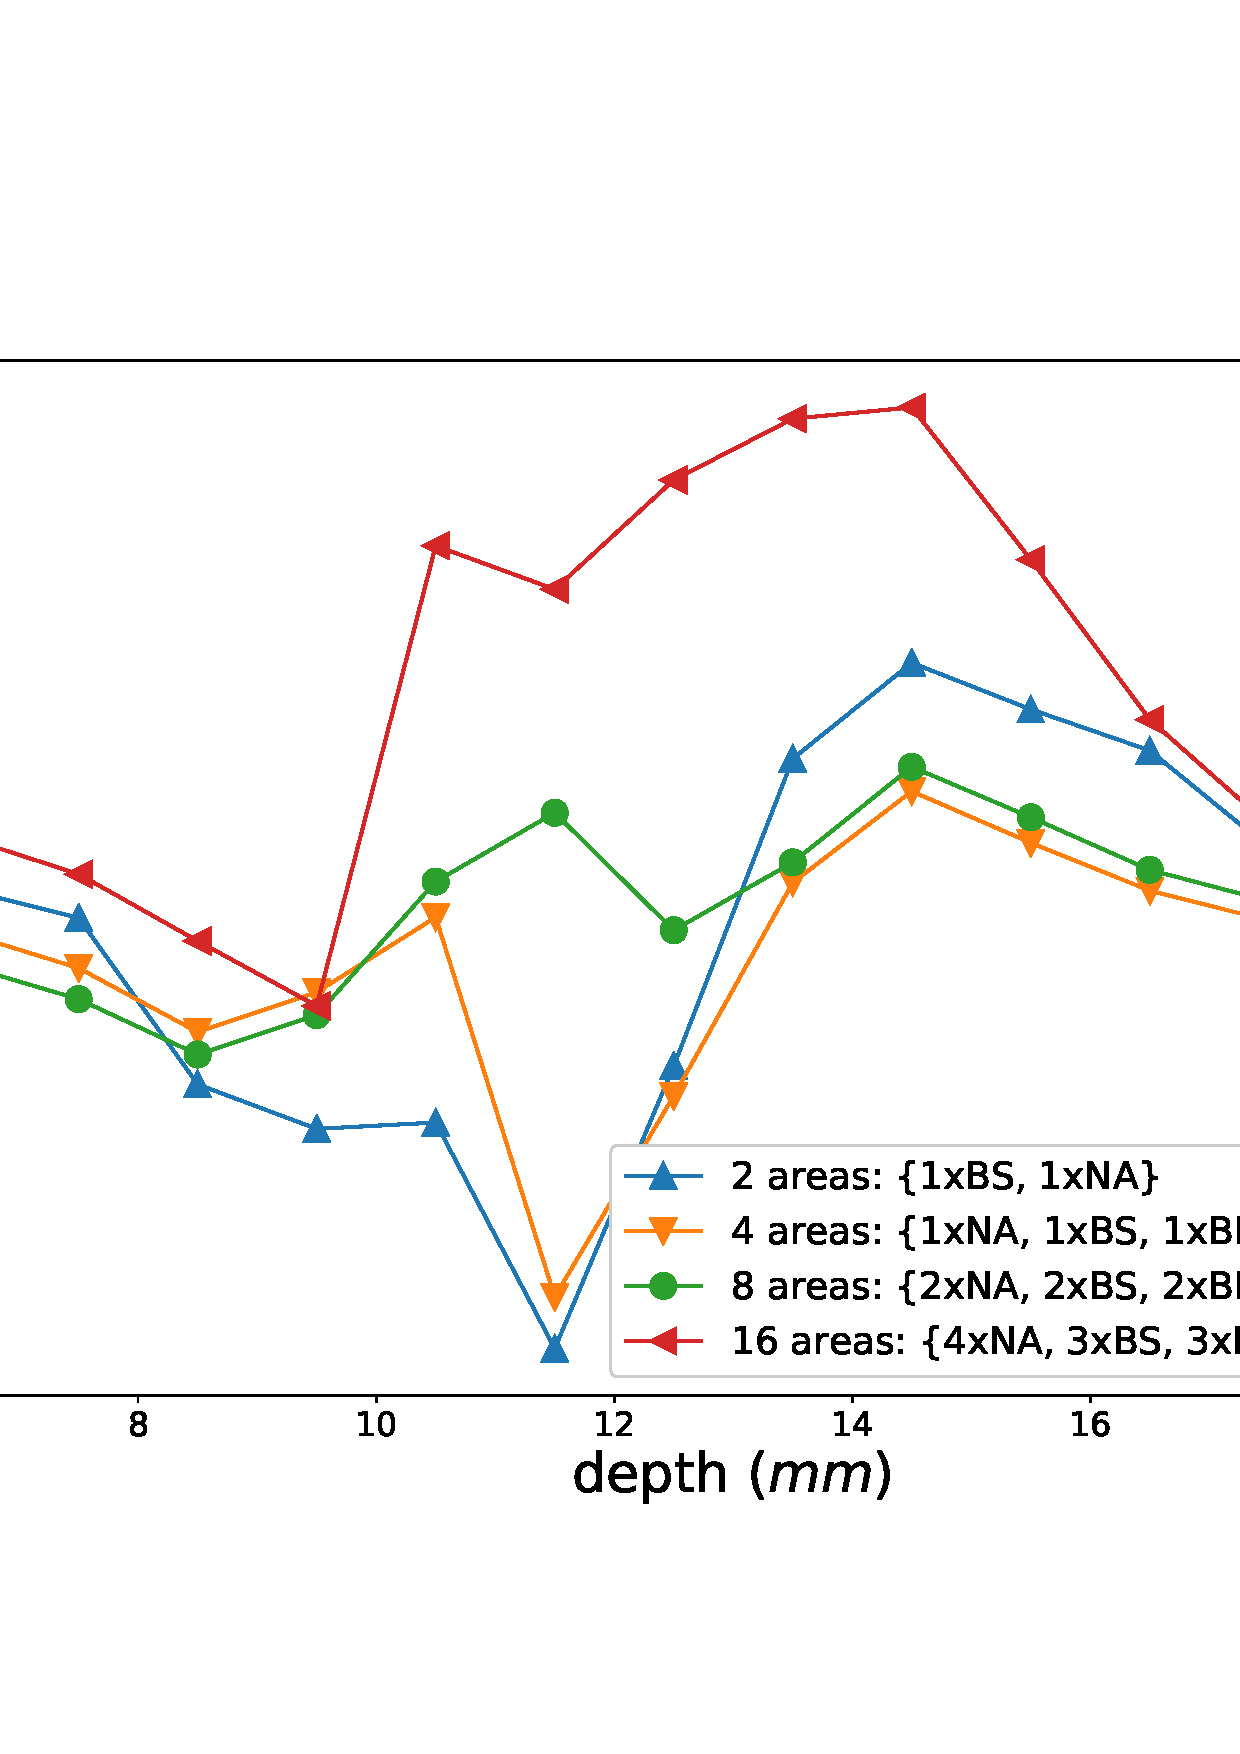
\includegraphics[width=\textwidth]{./figs/silhouette_coefficient_vertical_quantity.jpg}
			\caption{Vertical Motion}
			\label{silhouette_quantity:vertical}
		\end{subfigure}
		\begin{subfigure}[b]{.48\textwidth}
			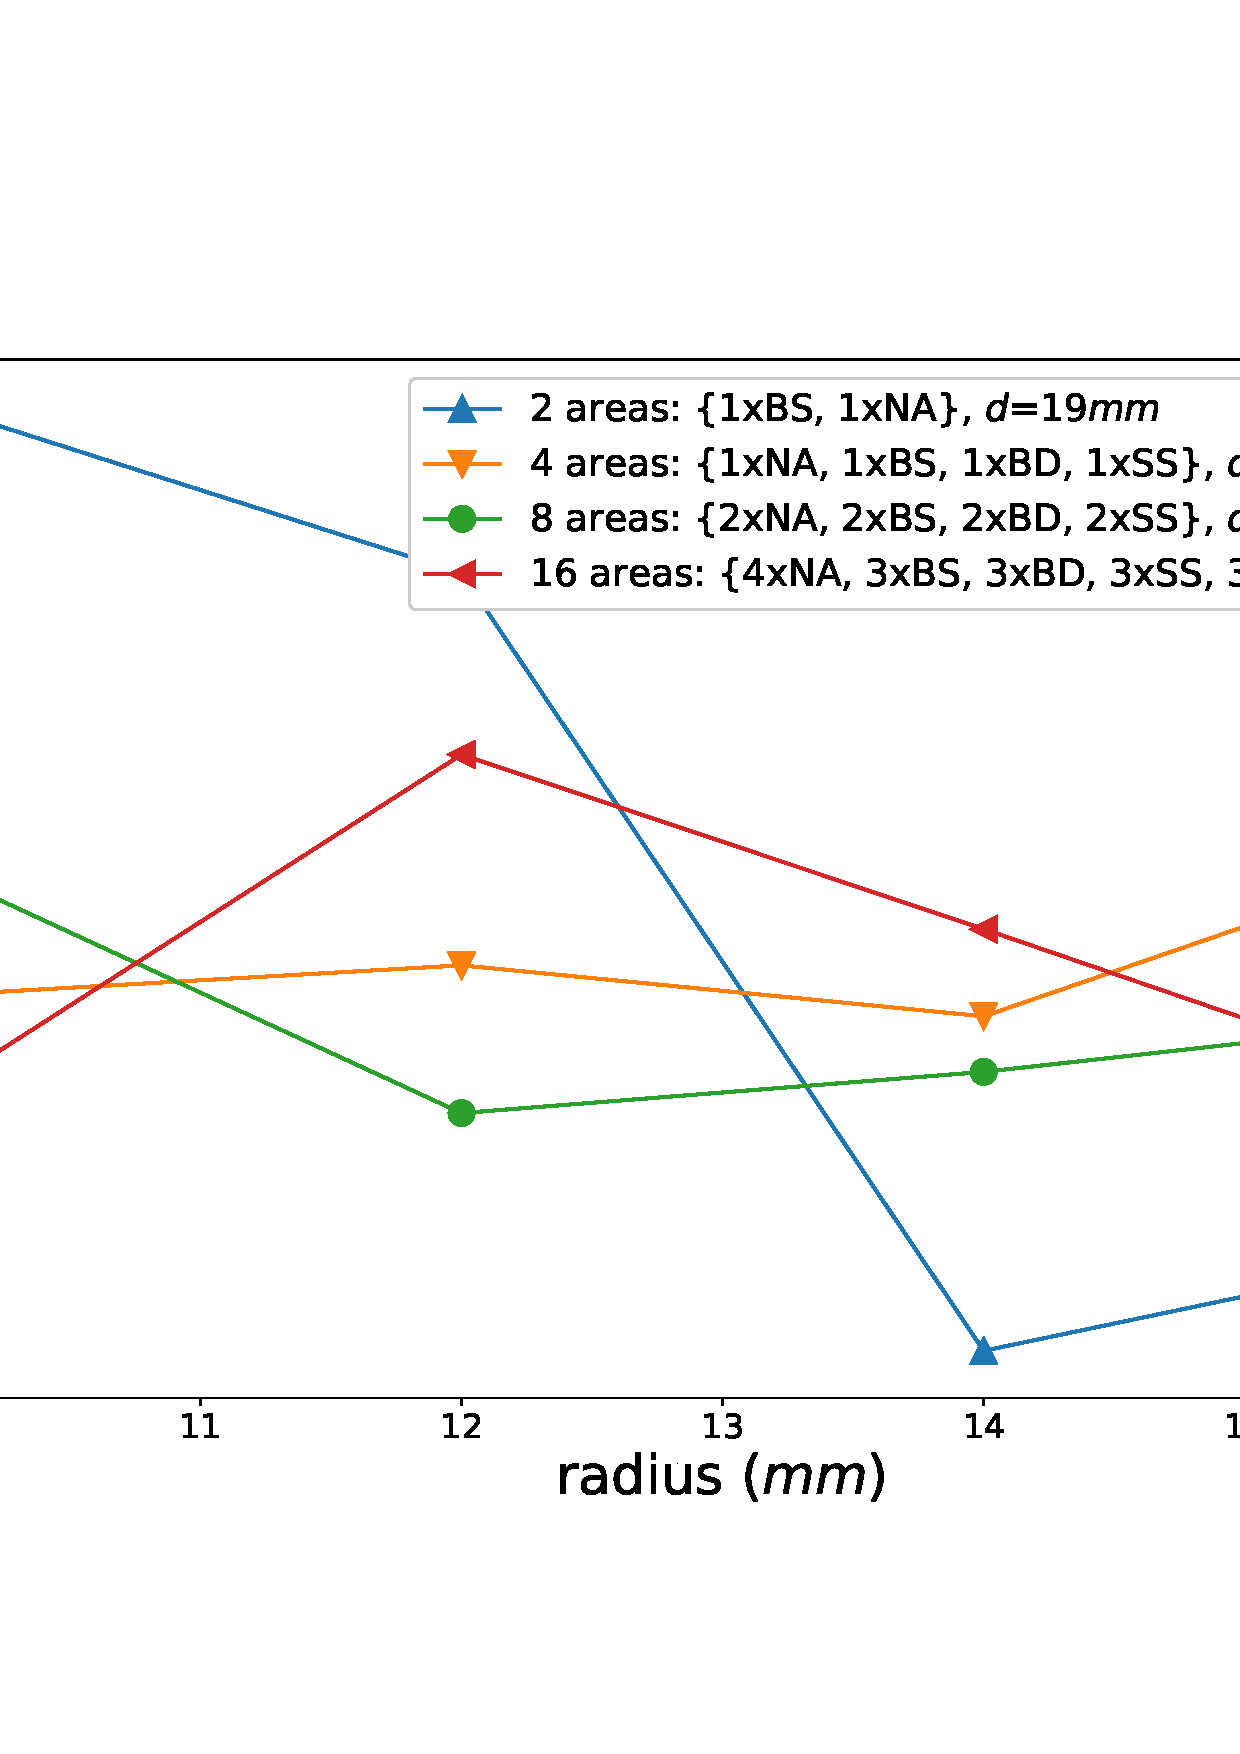
\includegraphics[width=\textwidth]{./figs/silhouette_coefficient_rotation_quantity.jpg}
			\caption{Rotatory Motion}
			\label{silhouette_quantity:Rotation}
		\end{subfigure}
		\caption{The figure show the change in silhouette coefficient by the 2D PCA subspace projection, when proving Vertically (a) and through the rotatory motion (b), changing the number of samples used to find the principal components ($N$ in $\mathbf{X}$, see Section \ref{sec_unsup_clustering}). }
		\label{silhouette_quantity}
	\end{figure}
	\begin{figure}[H]
		\centering
		\begin{subfigure}[b]{.48\textwidth}
			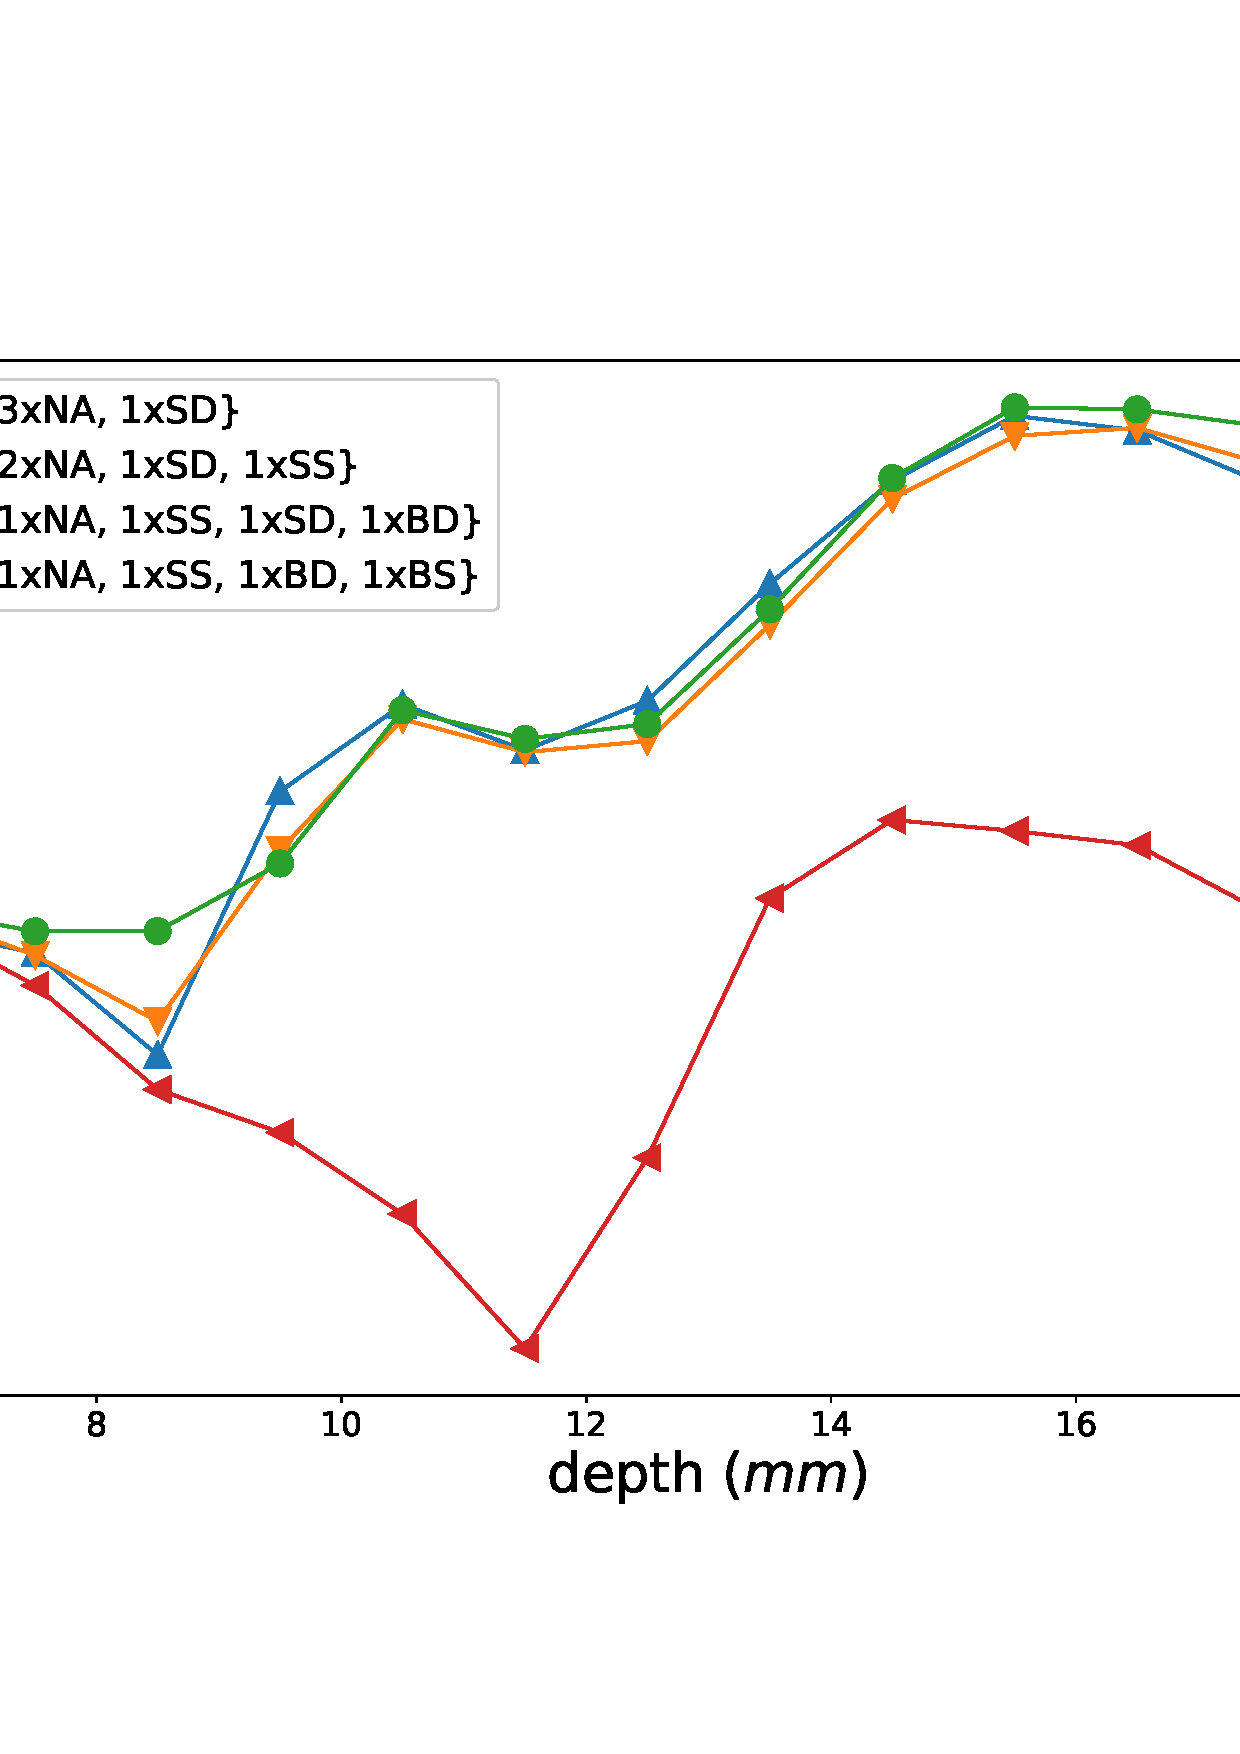
\includegraphics[width=\textwidth]{./figs/silhouette_coefficient_vertical_quality.jpg}
			\caption{Vertical Motion}
			\label{silhouette_quality:vertical}
		\end{subfigure}
		\begin{subfigure}[b]{.48\textwidth}
			\includegraphics[width=\textwidth]{./figs/silhouette_coefficient_rotation_quality.jpg}
			\caption{Rotatory Motion}
			\label{silhouette_quality:Rotation}
		\end{subfigure}
		\caption{The figure show the change in silhouette coefficient by the 2D PCA subspace projection, when proving Vertically (a) and through the rotatory motion (b), changing the quality of the samples used to find the principal components, while maintaining their number constant. }
		\label{silhouette_quality}
	\end{figure}
	\hfill\\
\end{minipage}


\begin{figure}[]
	\centering
	\includegraphics[width=.8\textwidth]{./figs/bar_clst_num_change}
	\caption{Silhouette Score of Vertical Motion, when changing the depth parameter, over different number of clusters.}
	\label{clst_number}
\end{figure}


%\begin{figure}[]
%	\centering
%	\begin{subfigure}[b]{.35\textwidth}
%		\includegraphics[width=\textwidth]{./figs/properties_cm_Rotate-d100-r100.jpg}
%		\caption{}
%		\label{ResRotcm:100-100}
%	\end{subfigure} 
%	\hspace{0.01\textwidth}
%	\begin{subfigure}[b]{0.35\textwidth}
%		\includegraphics[width=\textwidth]{./figs/properties_cm_Rotate-d100-r160.jpg}
%		\caption{}
%		\label{ResRotcm:100-160}
%	\end{subfigure}  
%	\hspace{0.01\textwidth}
%	\begin{subfigure}[b]{0.35\textwidth}
%		\includegraphics[width=\textwidth]{./figs/properties_cm_Rotate-d160-r100.jpg}
%		\caption{}
%		\label{ResRotcm:160-100}
%	\end{subfigure}
%	\hspace{0.01\textwidth}
%	\begin{subfigure}[b]{0.35\textwidth}
%		\includegraphics[width=\textwidth]{./figs/properties_cm_Rotate-d160-r160.jpg}
%		\caption{}
%		\label{ResRotcm:160-160}
%	\end{subfigure}
%	
%	\caption{Confusion matrices corresponding to the clustering results obtained with different parameters for the rotational movement. The diagonal in each matrix retains the counts for the correct cluster guesses.}
%	\label{ResRotcm}
%\end{figure}


\noindent We plot the accuracy and silhouette score for each tested combination of parameters in Fig. \ref{ResRotMetrics}. From the figure it is evident how both depth and rotation of motion aid in increasing performance over the task (Fig \ref{ResRotMetrics:acc}) and in obtaining higher quality clusters (Fig. \ref{ResVertAccMetrics:silhouette_score}) actively changing the information retrieved from the sensor to aid in future inference.

%\begin{figure}[]
%	\centering
%	\begin{subfigure}[b]{.48\textwidth}
%		\includegraphics[width=\textwidth]{./figs/phantom1propertiesRotate_accuracy.jpg}
%		\caption{}
%		\label{ResRotMetrics:ph1acc}
%	\end{subfigure}
%	\begin{subfigure}[b]{.48\textwidth}
%		\includegraphics[width=\textwidth]{./figs/phantom1propertiesRotate_silhouette.jpg}
%		\caption{}
%		\label{ResRotMetrics:ph1silhouette_score}
%	\end{subfigure}
%	\begin{subfigure}[b]{.48\textwidth}
%		\includegraphics[width=\textwidth]{./figs/phantom2propertiesRotate_accuracy.jpg}
%		\caption{}
%		\label{ResRotMetrics:ph2acc}
%	\end{subfigure}
%	\begin{subfigure}[b]{.48\textwidth}
%		\includegraphics[width=\textwidth]{./figs/phantom2propertiesRotate_silhouette.jpg}
%		\caption{}
%		\label{ResRotMetrics:ph2silhouette_score}
%	\end{subfigure}
%	\caption{Figure (a) and (b) show respectively the accuracy and the silhouette of the emerged categories when varying both the depth and rotation parameter of the rotatory motion primitive (see Section \ref{sec_experimental_protocol}), during interaction with phantom 1. Figure (c) and (d) show.. for phantom 2}
%	\label{ResRotMetrics}
%\end{figure}
 
\begin{figure}[]
	\centering
	\includegraphics[width=.75\textwidth]{./figs/phantom2propertiesVertical_na-dist}
	\caption{Distance of each cluster from the NA found cluster when changing the depth parameter of the Vertical motion.}
	\label{na_dist}
\end{figure}
 
\begin{figure}[]
	\centering
	\begin{subfigure}[b]{.48\textwidth}
		\includegraphics[width=\textwidth]{./figs/phantom1properties_distfig_Vertical-d6_5.jpg}
		\caption{}
		\label{cluster_distance:ph1-1}
	\end{subfigure}
	\begin{subfigure}[b]{.48\textwidth}
		\includegraphics[width=\textwidth]{./figs/phantom1properties_distfig_Vertical-d18_5.jpg}
		\caption{}
		\label{cluster_distance:ph1-2}
	\end{subfigure}
	\begin{subfigure}[b]{.48\textwidth}
		\includegraphics[width=\textwidth]{./figs/phantom2properties_distfig_Vertical-d6_5.jpg}
		\caption{}
		\label{cluster_distance:ph2-1}
	\end{subfigure}
	\begin{subfigure}[b]{.48\textwidth}
		\includegraphics[width=\textwidth]{./figs/phantom2properties_distfig_Vertical-d18_5.jpg}
		\caption{}
		\label{cluster_distance:ph2-2}
	\end{subfigure}
	\caption{Figure 10}
	\label{cluster_distance}
\end{figure}
 
 
%\begin{figure}[]
%	\centering
%	\begin{subfigure}[b]{.48\textwidth}
%		\includegraphics[width=\textwidth]{./figs/phantom1properties_tax-histogram_Vertical-d05.jpg}
%		\caption{}
%		\label{morphology:d0}
%	\end{subfigure}
%	\begin{subfigure}[b]{.48\textwidth}
%		\includegraphics[width=\textwidth]{./figs/phantom1properties_tax-histogram_Vertical-d185.jpg}
%		\caption{}
%		\label{morphology:d18}
%	\end{subfigure}
%	\caption{Figure (a) and (b) each show a histogram representing the tactile sensor used. For each bar, the height corresponds to the importance of the taxel in the corresponding position during the experiment.}
%	\label{morphology}
%\end{figure}
 
 
\subsection{Features of the Nodule (dimension, depth)}

We extend the probing by performing the experiments on a second phantom where we include a higher number of samples for each inclusion type (small-deep, small-superficial, big-deep, big-superficial \NoteP{need to say this better!! maybe mentioning ss, sd etc before and here just stating...}). We revise the Autonomous category formation process by changing the number of clusters to automatically find in the data from two to 5, and observe how the algorithm performs in the harder task of dissociating between the various type of inclusions. Thus, we change Equations \NoteP{(KMC EQUATION)} into \NoteP{NEW EQUATION}, and leave the remaining part of the process unchanged. 

RESULTS.

%
%\begin{figure}[]
%\centering
%\begin{subfigure}[b]{.48\textwidth}
%	\includegraphics[width=\textwidth]{./figs/properties_clsplt_Rotate-d100-r100.jpg}
%	\caption{}
%	\label{ResFeatRot:100-100}
%\end{subfigure} 
%\hspace{0.01\textwidth}
%\begin{subfigure}[b]{0.48\textwidth}
%	\includegraphics[width=\textwidth]{./figs/properties_clsplt_Rotate-d100-r160.jpg}
%	\caption{}
%	\label{ResFeatRot:100-160}
%\end{subfigure}
%\hspace{0.01\textwidth}
%\begin{subfigure}[b]{0.48\textwidth}
%	\includegraphics[width=\textwidth]{./figs/properties_clsplt_Rotate-d160-r100.jpg}
%	\caption{}
%	\label{ResFeatRot:160-100}
%\end{subfigure}
%\hspace{0.01\textwidth}
%\begin{subfigure}[b]{0.48\textwidth}
%	\includegraphics[width=\textwidth]{./figs/properties_clsplt_Rotate-d160-r160.jpg}
%	\caption{}
%	\label{ResFeatRot:160-160}
%\end{subfigure}
%
%\caption{The Figure shows the 5-dimensional projection
%	of different combination of depth and radius on the two axis of highest variance in the data for rotational movement (a) $depth = 10mm$, $radius = 10mm$  (b) $depth = 10mm$, $radius = 16mm$ (c) $depth = 16mm$, $radius = 10mm$ (d) $depth = 16mm$, $radius = 16mm$. The line $l_{kmc}$ corresponds to the decision boundary of the two cluster as found by the KMC algorithm, and C0, C1, C2, C3, C4 their corresponding centroids.}
%\label{ResFeatRot}
%\end{figure} 	



%\begin{figure}[]
% 	\centering
% 	\begin{subfigure}[b]{.35\textwidth}
% 		\includegraphics[width=\textwidth]{./figs/properties_cm_Rotate-d100-r100.jpg}
% 		\caption{}
% 		\label{ResRotfeatcm:100100}
% 	\end{subfigure} 
% 	\hspace{0.01\textwidth}
% 	\begin{subfigure}[b]{0.35\textwidth}
% 		\includegraphics[width=\textwidth]{./figs/properties_cm_Rotate-d100-r160.jpg}
% 		\caption{}
% 		\label{ResRotfeatcm:100160}
% 	\end{subfigure}  
% 	\hspace{0.01\textwidth}
% 	\begin{subfigure}[b]{0.35\textwidth}
% 		\includegraphics[width=\textwidth]{./figs/properties_cm_Rotate-d160-r100.jpg}
% 		\caption{}
% 		\label{ResRotfeatcm:160100}
% 	\end{subfigure}
% 	\hspace{0.01\textwidth}
% 	\begin{subfigure}[b]{0.35\textwidth}
% 		\includegraphics[width=\textwidth]{./figs/properties_cm_Rotate-d160-r160.jpg}
% 		\caption{}
% 		\label{ResRotfeatcm:160160}
% 	\end{subfigure}
% 	
% 	\caption{Confusion matrices corresponding to the clustering results obtained with different parameters for the rotational movement. The diagonal in each matrix retains the counts for the correct cluster guesses.}
% 	\label{ResRotfeatcm}
%\end{figure}
%
%\begin{figure}[]
%  	\centering
%  	\begin{subfigure}[b]{.48\textwidth}
%  		\includegraphics[width=\textwidth]{./figs/properties_clsplt_Vertical-dn0-NA.jpg}
%  		\caption{}
%  		\label{ResfeatVert:dn0}
%  	\end{subfigure} 
%  	\hspace{0.01\textwidth}
%  	\begin{subfigure}[b]{0.48\textwidth}
%  		\includegraphics[width=\textwidth]{./figs/properties_clsplt_Vertical-dn6-NA.jpg}
%  		\caption{}
%  		\label{ResfeatVert:dn9}
%  	\end{subfigure}
%  	
%  	\caption{The Figure shows the 2-dimensional projection
%  		of min and max depthon the two axis of highest variance in the
%  		data for vertical movement (a) $depth = 0.5mm$ (b) $depth = 18.5mm$. The line $l_{kmc}$ corresponds to the decision boundary of the two cluster as found by the KMC algorithm, and C0 and C1 their corresponding centroids.}
%  	\label{ResfeatVert}
%\end{figure}


%\begin{figure}[]
%  	\centering
%  	\begin{subfigure}[b]{.35\textwidth}
%  		\includegraphics[width=\textwidth]{./figs/properties_cm_Vertical-dn0-NA.jpg}
%  		\caption{}
%  		\label{Resfeatvertcm:dn0}
%  	\end{subfigure} 
%  	\hspace{0.01\textwidth}
%  	\begin{subfigure}[b]{0.35\textwidth}
%  		\includegraphics[width=\textwidth]{./figs/properties_cm_Vertical-dn6-NA.jpg}
%  		\caption{}
%  		\label{Resfeatvertcm:dn9}
%  	\end{subfigure}  
%  	\caption{Confusion matrices corresponding to the clustering results obtained with different parameters for the vertical movement. The diagonal in each matrix retains the counts for the correct cluster guesses.}
%  	\label{Resfeatvertcm}
%\end{figure}
 	  
\section{Discussion} 	\label{sec_discussion}
Like previously mentioned, sensory motor coordination is a fundamental skill in many biological organisms and one that we wish to exploit in full in robotics. Actively choosing an interaction strategy to optimize sensory perception for a specific task at hand has the potential to be a most powerful tool, endowing robots with the ability to dynamically filter, thus choose to perceive, some stimuli rather then others, essentially solving in part the task before the sensory stimuli arrive to a central processing unit. 

Observing the changing in tactile encoding through the Autonomous Category Formation lens has allowed us to see how a set of motion primitives effected the sensory information of each probed location in a soft phantom, without influencing inference in any way (due to the unsupervised nature of the process). From the two utilized motions it is clear how a more involved motion strategy, such as the rotary motion, allows for better hard inclusion classification. The radius of rotation in the rotary primitive motion, in fact, allows the robot to retrieve a more complex and rich sensor time series response over the duration of the motion. The changed sensor response, then, is shown to fire for hard inclusions, even when these are far below the surface of the soft body. More interestingly, however, is the change in information obtained when varying the depth of probing for both the motion primitives employed. This, in fact, not only causes the sensor's response to saturate better over areas with hard inclusions, but unifies the sensor response for areas where no hard inclusion is detected, effectively increasing its certainty over these. 

DISCUSSION OVER INCLUSION PROPERTIES EXTENSION


\section{Conclusions} \label{sec_conclusion}
Sensory motor coordination is a fundamental process by which the sensory inputs can be actively changed by interactions with the environment. In the context of detecting hard inclusions in a soft body by means of a capacitive tactile sensor, we wish to investigate the effects of various motion strategies to the sensor response, and consequently to the robot's perception of stimuli through their categorization. After proposing an Autonomous Category Formation process to group stimuli into clusters, we embed a capacitive tactile sensor onto an 3D-printed end-effector, and probe a phantom with various hard inclusions through different motion strategies. We explore two motion strategies: Vertical and Rotary. The sequential sensor data obtained through the probing of each area in the phantom is clustered, and the change in information due to each motion strategy is observed. We find the robot capable of finding large inclusions (DIMENSION) both when superficial (\NoteP{depth}) or deep \NoteP{depth} in the soft body, while smaller inclusions (\NoteP{size}), if detectable at \NoteP{depth}, can not be distinguished from empty areas when at grated depths. The rotary motion strategy performs better in general, due to the richer information retrieved over time when probing for hard inclusions. We find the radius of rotation important in retrieving information relative to a hard nodule when one is found. More interestingly, we find depth to, not only change the sensor response to fire for hard inclusion, but to coalesce the response for empty areas, increasing certainty of emptiness for the same.




% \begin{table}
% \tbl{Example of a table showing that its caption is as wide as
%  the table itself and justified.}
% {\begin{tabular}{lcccccc} \toprule
%  & \multicolumn{2}{l}{Type} \\ \cmidrule{2-7}
%  Class & One & Two & Three & Four & Five & Six \\ \midrule
%  Alpha\textsuperscript{a} & A1 & A2 & A3 & A4 & A5 & A6 \\
%  Beta & B2 & B2 & B3 & B4 & B5 & B6 \\
%  Gamma & C2 & C2 & C3 & C4 & C5 & C6 \\ \bottomrule
% \end{tabular}}
% \tabnote{\textsuperscript{a}This footnote shows how to include
%  footnotes to a table if required.}
% \label{sample-table}
% \end{table}

% \subsection{Landscape pages}

% If a figure or table is too wide to fit the page it will need to be rotated, along with its caption, through 90$^{\circ}$ anticlockwise. Landscape figures and tables can be produced using the \verb"rotating" package, which is called by the \texttt{interact} class file. The following commands (for example) can be used to produce such pages.

% Before any such float environment, use the \verb"\setcounter" command as above to fix the numbering of the caption (the value of the counter being the number given to the preceding figure or table). Subsequent captions will then be automatically renumbered accordingly. The \verb"\epsfbox" command requires \verb"epsfig.sty", which is called by the \texttt{interact} class file and is also included in the \textsf{Interact} \LaTeX\ bundle for convenience.

% Note that if the \verb"endfloat" package is used, one or both of the commands
% \begin{verbatim}
% \DeclareDelayedFloatFlavor{sidewaysfigure}{figure}
% \DeclareDelayedFloatFlavor{sidewaystable}{table}
% \end{verbatim}
% will need to be included in the preamble of your .tex file, after the \verb"endfloat" package is loaded, in order to process any landscape figures and/or tables correctly.




\section*{Acknowledgement(s)}

An unnumbered section, e.g.\ \verb"\section*{Acknowledgements}", may be used for thanks, etc.\ if required and included \emph{in the non-anonymous version} before any Notes or References.


\bibliographystyle{tfnlm}
\bibliography{IEEEexample}


\bigskip


\end{document}
